\documentclass{report}
\usepackage{authblk}
\usepackage{mathptmx}
\usepackage{url,latexsym,amsmath,amsthm,xspace,rotating,multirow,multicol,xspace,amssymb,paralist}
\usepackage{euscript}
\usepackage{fancybox,xcolor}
\usepackage{longtable}
\usepackage{paralist}
\usepackage[normalem]{ulem}
\usepackage[pdftex]{hyperref}
\usepackage{algorithmicx}
\usepackage{algpseudocode}
\usepackage{algorithm}
\usepackage{cancel}
\usepackage{mathtools}

\usepackage{url}
\usepackage{latexsym}

\usepackage{times}
\usepackage{amsmath}
\usepackage{amsthm}
\usepackage{amssymb}
\usepackage{graphicx}
\usepackage{xspace}
\usepackage{tabularx}
\usepackage{multicol}
\usepackage{multirow}
%\usepackage{hyperref}
\usepackage{url}
%\usepackage{natbib}
\usepackage{wrapfig}
\usepackage{comment}
\usepackage{listings}
\usepackage{color}
\usepackage[utf8]{inputenc}
\usepackage{fancyvrb}
\usepackage{booktabs}
\usepackage{color}
\usepackage[normalem]{ulem}

\newcommand{\obs}{\text{obs}}
\newcommand{\mis}{\text{mis}}

\newcommand{\qt}[1]{\left<#1\right>}
\newcommand{\ql}[1]{\left[#1\right]}
\newcommand{\hess}{\mathbf{H}}
\newcommand{\jacob}{\mathbf{J}}
\newcommand{\hl}{HL}
\newcommand{\cost}{\mathcal{L}}
\newcommand{\lout}{\mathbf{r}}
\newcommand{\louti}{r}
\newcommand{\outi}{y}
\newcommand{\out}{\mathbf{y}}
\newcommand{\gauss}{\mathbf{G_N}}
\newcommand{\eye}{\mathbf{I}}
\newcommand{\softmax}{\text{softmax}}
\newcommand{\targ}{\mathbf{t}}
\newcommand{\metric}{\mathbf{G}}
\newcommand{\sample}{\mathbf{z}}
\newcommand{\f}{\text{f}}
%\newcommand{\log}{\text{log}}

\newcommand{\bmx}[0]{\begin{bmatrix}}
\newcommand{\emx}[0]{\end{bmatrix}}
\newcommand{\qexp}[1]{\left<#1\right>}
\newcommand{\vect}[1]{\mathbf{#1}}
\newcommand{\vects}[1]{\boldsymbol{#1}}
\newcommand{\matr}[1]{\mathbf{#1}}
\newcommand{\var}[0]{\operatorname{Var}}
\newcommand{\std}[0]{\operatorname{std}}
\newcommand{\cov}[0]{\operatorname{Cov}}
\newcommand{\diag}[0]{\operatorname{diag}}
\newcommand{\matrs}[1]{\boldsymbol{#1}}
\newcommand{\va}[0]{\vect{a}}
\newcommand{\vb}[0]{\vect{b}}
\newcommand{\vc}[0]{\vect{c}}
\newcommand{\ve}[0]{\vect{e}}

\newcommand{\vh}[0]{\vect{h}}
\newcommand{\vv}[0]{\vect{v}}
\newcommand{\vx}[0]{\vect{x}}
\newcommand{\vp}[0]{\vect{p}}
\newcommand{\vz}[0]{\vect{z}}
\newcommand{\vw}[0]{\vect{w}}
\newcommand{\vs}[0]{\vect{s}}
\newcommand{\vf}[0]{\vect{f}}
\newcommand{\vi}[0]{\vect{i}}
\newcommand{\vo}[0]{\vect{o}}
\newcommand{\vd}[0]{\vect{d}}
\newcommand{\vy}[0]{\vect{y}}
\newcommand{\vg}[0]{\vect{g}}
\newcommand{\vm}[0]{\vect{m}}
\newcommand{\vu}[0]{\vect{u}}
\newcommand{\vL}[0]{\vect{L}}
\newcommand{\vr}[0]{\vect{r}}
\newcommand{\vone}[0]{\vect{1}}

\newcommand{\mW}[0]{\matr{W}}
\newcommand{\mE}[0]{\matr{E}}
\newcommand{\mG}[0]{\matr{G}}
\newcommand{\mX}[0]{\matr{X}}
\newcommand{\mY}[0]{\matr{Y}}
\newcommand{\mQ}[0]{\matr{Q}}
\newcommand{\mU}[0]{\matr{U}}
\newcommand{\mF}[0]{\matr{F}}
\newcommand{\mV}[0]{\matr{V}}
\newcommand{\mA}{\matr{A}}
\newcommand{\mC}{\matr{C}}
\newcommand{\mD}{\matr{D}}
\newcommand{\mL}[0]{\matr{L}}
\newcommand{\mR}[0]{\matr{R}}
\newcommand{\mS}{\matr{S}}
\newcommand{\mI}{\matr{I}}
\newcommand{\td}[0]{\text{d}}
\newcommand{\TT}[0]{\vects{\theta}}
\newcommand{\vsig}[0]{\vects{\sigma}}
\newcommand{\valpha}[0]{\vects{\alpha}}
\newcommand{\vmu}[0]{\vects{\mu}}
\newcommand{\vzero}[0]{\vect{0}}
\newcommand{\tf}[0]{\text{m}}
\newcommand{\tdf}[0]{\text{dm}}
\newcommand{\grad}[0]{\nabla}
\newcommand{\alert}[1]{\textcolor{red}{#1}}
\newcommand{\N}[0]{\mathcal{N}}
\newcommand{\YY}[0]{\mathcal{Y}}
\newcommand{\BB}[0]{\mathcal{B}}
\newcommand{\LL}[0]{\mathcal{L}}
\newcommand{\HH}[0]{\mathcal{H}}
\newcommand{\RR}[0]{\mathbb{R}}
\newcommand{\MM}[0]{\mathcal{M}}
\newcommand{\OO}[0]{\mathbb{O}}
\newcommand{\II}[0]{\mathbb{I}}
\newcommand{\Scal}[0]{\mathcal{S}}
\newcommand{\sigmoid}{\sigma}
\newcommand{\sign}{\text{sign}}
\newcommand{\E}[0]{\mathbb{E}}
\newcommand{\enabla}[0]{\ensuremath{%
    \overset{\raisebox{-0.3ex}[0.5ex][0ex]{%
    \ensuremath{\scriptscriptstyle e}}}{\nabla}}}
\newcommand{\enhnabla}[0]{\nabla_{\hspace{-0.5mm}e}\,}
\newcommand{\eos}[0]{\ensuremath{\left< \text{eos}\right>}}


\newcommand{\todo}[1]{{\Large\textcolor{red}{#1}}}
\newcommand{\done}[1]{{\Large\textcolor{green}{#1}}}
\newcommand{\dd}[1]{\ensuremath{\mbox{d}#1}}

\DeclareMathOperator*{\argmax}{\arg \max}
\DeclareMathOperator*{\argmin}{\arg \min}
\newcommand{\newln}{\\&\quad\quad{}}

\newcommand{\BP}{\text{BP}}
\newcommand{\PPL}{\text{PPL}}
\newcommand{\PL}{\text{PL}}
\newcommand{\MatSum}{\text{MatSum}}
\newcommand{\MatMul}{\text{MatMul}}
\newcommand{\KL}{\text{KL}}
\newcommand{\data}{\text{data}}
\newcommand{\rect}{\text{rect}}
\newcommand{\maxout}{\text{maxout}}
\newcommand{\train}{\text{train}}
\newcommand{\hinge}{\text{hinge}}
\newcommand{\val}{\text{val}}
\newcommand{\init}{\text{init}}
\newcommand{\fenc}{\text{fenc}}
\newcommand{\renc}{\text{renc}}
\newcommand{\enc}{\text{enc}}
\newcommand{\dec}{\text{dec}}
\newcommand{\test}{\text{test}}
\newcommand{\tra}{\text{tra}}
\newcommand{\Ax}{\mathcal{A}_x}
\newcommand{\Ay}{\mathcal{A}_y}
\newcommand{\ola}{\overleftarrow}
\newcommand{\ora}{\overrightarrow}
\newcommand{\ov}{\overline}
\newcommand{\ts}{\rule{0pt}{2.6ex}}       % Top strut
\newcommand{\ms}{\rule{0pt}{0ex}}         % Middle strut
\newcommand{\bs}{\rule[-1.2ex]{0pt}{0pt}} % Bottom strut
\newcommand{\specialcell}[2][c]{%
  \begin{tabular}[#1]{@{}c@{}}#2\end{tabular}}


%\usepackage{bibentry}
%\nobibliography*

\begin{document}

\title{Introduction to Machine Learning}
\author{Kyunghyun Cho}
\affil{
    Courant Institute of Mathematical Sciences and \\
    Center for Data Science,\\
    New York University 
}

\maketitle
\pagenumbering{arabic}

\abstract{
    This is a lecture note for the course CSCI-UA.0473-001 (Intro to Machine
    Learning) at the Department of Computer Science, Courant Institute of
    Mathematical Sciences at New York University. The content of the lecture
    note was selected to fit a single 12-week-long course (3 hours a week) and
    to mainly serve undergraduate students majoring in computer science. Many
    existing materials in machine learning therefore had to be omitted. 
    
    For a more complete coverage of machine learning (with math!), the following
    text books are recommended in addition to this lecture note:
    \begin{itemize}
        \item ``Pattern Recognition and Machine Learning'' by Chris Bishop \cite{bishop2006pattern}
        \item ``Machine Learning: a probabilistic perspective'' by Kevin Murphy \cite{murphy2012machine}
        \item ``A Course in Machine Learning'' by Hal Daum\'e\footnote{
                Available at \url{http://ciml.info/}.
            }
    \end{itemize}

    For practical exercises, Python scripts based on numpy and scipy are
    available at
    \url{https://github.com/nyu-dl/Intro_to_ML_Lecture_Note/tree/master/notebook}.
    They are under heavy development and subject to frequent changes over the
    course. I recommend you to check back frequently. Again, these are not
    exhaustive, and for a more complete coverage on machine learning practice, I
    recommend the following book:
    \begin{itemize}
        \item ``Introduction to Machine Learning with Python'' by Andreas
            M\"uller  and Sarah Guido
    \end{itemize}

    Note that those sections marked with $\star$ are optional and will not be
    covered during regular lectures. They will likely not be filled in by the
    end of the first round of the lectures either.. 
}

\chapter*{Notations}

Throughout this lecture note, I will use the following notational conventions:
\begin{itemize}
    \item A bold-faced lower-case alphabet is used for a vector: $\vx$
    \item A bold-faced upper-case alphabet is used for a matrix: $\mW$
    \item A lower-case alphabet is often used for a scalar: $x$, $\eta$
    \item A lower-case alphabet is also used for denoting a function
    \item 
\end{itemize}


\chapter{Classification}
\label{sec:classification}

\section{Supervised Learning}
\label{sec:supervised_learning}

In supervised learning, our goal is to build or find a machine $M$ that takes as
input a multi-dimensional vector $\vx \in \mathbb{R}^d$ and outputs a response
vector $\vy \in \mathbb{R}^{d'}$.  That is,
\begin{align*}
    M: \mathbb{R}^d \to \mathbb{R}^{d'}.
\end{align*}
Of course this cannot be done out of blue, and we first assume that there exists
a reference design $M^*$ of such a machine.  We then refine our goal as to build
or find a machine $M$ that imitates the reference machine $M^*$ as closely as
possible. In other words, we want to make sure that for any given $\vx$, the
outputs of $M$ and $M^*$ coincide, i.e.,
\begin{align}
    \label{eq:classification0}
    M(\vx) = M^*(\vx),\text{ for all } \vx \in \mathbb{R}^d.
\end{align}
This is still not enough for us to find $M$, because there are infinitely many
possible $M$'s through which we must search. We must hence decide on our {\it
hypothesis set} $H$ of potential machines. This is an important decision, as it
directly influences the difficulty in finding such a machine. When your
hypothesis set is not constructed well, there may not be a machine that
satisfies the criterion above. 

We can state the same thing in a slightly different way. First, let us assume a
function $D$ that takes as input the output of $M^*$, a machine $M$ and an input
vector $\vx$, and returns how much they differ from each other, i.e.,
\begin{align*}
    D: \mathbb{R}^{d'} \times H \times \mathbb{R}^{d'} \to \mathbb{R}_+,
\end{align*}
where $\mathbb{R}_+$ is a set of non-negative real numbers. As usual in our
everyday life, the smaller the output of $D$ the more similar the outputs of $M$
and $M^*$. An example of such a function would be
\begin{align*}
    D(y, M, \vx) = \left\{
        \begin{array}{l l}
            0, & \text{if }  y = M(\vx) \\
            1, & \text{otherwise}
        \end{array}
        \right..
\end{align*}

It is certainly possible to tailor this distance function, or a {\it
per-example cost} function, for a specific target task. For instance, consider
an intrusion detection system $M$ which takes as input a video frame of a store
front and returns a binary indicator, instead of a real number, whether there is
a thief in front of the store (0: no and 1: yes). When there is no thief
($M^*(\vx)=0$), it does not cost you anything when $M$ agrees with $M^*$, but
you must pay \$10 for security dispatch if $M$ predicted $1$. When there is a
thief in front of your store ($M^*(\vx)=1$), you will lose \$100 if the alarm
fails to detect the thief ($M(\vx)=0$) but will not lose any if the alarm went
off. In this case, we may define the per-example cost function as
\begin{align*}
    D(y, M, \vx) = \left\{
        \begin{array}{l l}
            0, & \text{if }  y=M(\vx) \\
            -10, & \text{if }  y=0\text{ and }M(\vx)=1 \\
            -100, & \text{if }  y=1\text{ and }M(\vx)=0 
        \end{array}
        \right..
\end{align*}
Note that this distance is asymmetric.

Given a distance function $D$, we can now state the supervised learning
problem as finding a machine $M$, with in a given hypothesis set $H$, that
minimizes its distance from the reference machine $M^*$ for any given input.
That is,
\begin{align}
    \label{eq:classification1}
    \argmin_{M \in H} \int_{\mathbb{R}^d} D(M^*(\vx), M, \vx) \text{d}\vx.
\end{align}

You may have noticed that these two conditions in
Eqs.~\eqref{eq:classification0}--\eqref{eq:classification1} are not equivalent.
If a machine $M$ satisfies the first condition, the second conditions is
naturally satisfied. The other way around however does not necessarily hold.
Even then, we prefer the second condition as our ultimate goal to satisfy in
machine learning. This is because we often cannot guarantee that $M^*$ is
included in the hypothesis set $H$. The first condition simple becomes
impossible to satisfy when $M^* \notin H$, but the second condition gets us a
machine $M$ that is {\it close} enough to the reference machine $M^*$. We prefer
to have a suboptimal solution rather than having no solution.

The formulation in Eq.~\eqref{eq:classification1} is however not satisfactory.
Why? Because not every point $\vx$ in the input space $\mathbb{R}^d$ is born
equal. Let us consider the previous example of a video-based intrusion detection
system again. Because the camera will be installed in a fixed location pointing toward
the store front, video frames will generally look similar to each other, and
will only form a very small subset of all possible video frames, unless some
exotic event happens. In this case, we would only care whether our alarm $M$
works well for those frames showing the store front and people entering or
leaving the store. Whether the distance between the reference machine and my
alarm is small for a video frame showing the earth from the outer space would
not matter at all.

And, here comes probability. We will denote by $p_X(\vx)$ the probability
(density) assigned to the input $\vx$ under the distribution $X$, and assume
that this probability reflects how likely the input $\vx$ is. We want to
emphasize the impact of the distance $D$ on likely inputs (high $p_X(\vx)$)
while ignoring the impact on unlikely inputs (low $p_X(\vx)$). In other words,
we weight each per-example cost with the probability of the corresponding
example. Then the problem of supervised learning becomes 
\begin{align}
    \label{eq:expected_loss0}
    \argmin_{M\in H} \int_{\mathbb{R}^d} p_X(\vx) D(M^*(\vx), M, \vx) \text{d}\vx 
    = \argmin_{M \in H} \mathbb{E}_{\vx \sim X} \left[ D(M^*(\vx),  M, \vx)
    \right].
\end{align}

Are we done yet? No, we still need to consider one more hidden cost in order to
make the description of supervised learning more complete. This hidden cost
comes from the operational cost, or {\it complexity}, of each machine $M$ in the
hypothesis set $H$.  It is reasonable to think that some machines are cheaper or
more desirable to use than some others are. Let us denote this cost of a machine
by $C(M)$, where $C: H \to \mathbb{R}_+$. Our goal is now slightly more
complicated in that we want to find a machine that minimizes both the cost in
Eq.~\eqref{eq:expected_loss0} and its operational cost. So, at the end, we get
\begin{align}
    \label{eq:expected_loss1}
    \argmin_{M \in H} \underbrace{\mathbb{E}_{\vx \sim X} \left[ D(M^*(\vx), M, \vx) \right]
        + \lambda C(M)
    }_{
        \mathclap{R = \text{Expected Cost}}
    },
\end{align}
where $\lambda \in \mathbb{R}_+$ is a coefficient that trades off the importance
between the expected distance (between $M^*$ and $M$) and the operational cost
of $M$.

In summary, supervised learning is a problem of finding a machine $M$ such that
has bot the low expectation of the distance between the outputs of $M^*$ and
$M$ over the input distribution and the low operational cost.

\paragraph{In Reality}

It is unfortunately impossible to solve the minimization problem in
Eq.~\eqref{eq:expected_loss1} in reality. There are so many reasons behind this,
but the most important reason is the input distribution $p_X$ or lack thereof.
We can decide on a distance function $D$ ourselves based on our goal. We can
decide ourselves a hypothesis set $H$ ourselves based on our requirements and
constraints. All good, but $p_X$ is not controllable in general, as it reflects
how the world is, and the world does not care about our own requirements nor
constraints.  

Let's take the previous example of video-based intrusion system. Our reference
machine $M^*$ is a security expert who looks at a video frame (and a person
within it) and determines whether that person is an intruder. We may decide to
search over any arbitrary set of neural networks to minimize the expected loss.
We have however absolutely no idea what the precise probability $p(\vx)$ of any
video frame. Instead, we only observe $\vx$'s which was randomly sampled from
the input distribution by the surrounding environment. We have no access to the
input distribution itself, but what comes out of it. 

We only get to observe a {\it finite} number of such samples $\vx$'s, with which
we must approximate the expected cost in Eq.~\eqref{eq:expected_loss1}. This
approximation method, that is approximation based on a finite set of samples
from a probability distribution, is called a {\it Monte Carlo method}.  Let us
assume that we have observed $N$ such samples: $\left\{ \vx^1, \ldots, \vx^N
\right\}$. Then we can approximate the expected cost by
\begin{align}
    \label{eq:empirical_loss}
    \underbrace{\mathbb{E}_{\vx \sim X} \left[ D(M^*(\vx), M, \vx) \right] +
    \lambda C(M)}_{
        \mathclap{\text{Expected Cost}}
    } =
    \underbrace{
        \frac{1}{N} \sum_{n=1}^N D(M^*(\vx^n), M, \vx^n)
        + \lambda C(M)
    }_{\mathclap{\tilde{R} = \text{Empirical Cost}}} + \epsilon,
\end{align}
where $\epsilon$ is an approximation error. We will call this cost, computed
using a finite set of input vectors, an {\it empirical cost}. 

\paragraph{Inference}

We have so far talked about what is a correct way to find a machine $M$ for our
purpose. We concluded that we want to find $M$ by minimizing the empirical cost
in Eq.~\eqref{eq:empirical_loss}. This is a good start, but let's discuss why we
want to do this first. There may be many reasons, but often a major complication
is the expense of running the reference machine $M^*$ or the limited access to
the reference machine $M^*$. Let us hence make it more realistic by assuming
that we will have access to $M^*$ only once at the very beginning together with
a set of input examples. In other words, we are given
\begin{align*}
    D_{\text{tra}} = \left\{ (\vx^1, M^*(\vx^1)), \ldots, (\vx^N,
    M^*(\vx^N))\right\},
\end{align*}
to which we refer as a {\it training set}. Once this set is available, we can
find $M$ that minimizes the empirical cost from Eq.~\eqref{eq:empirical_loss}
without ever having to query the reference machine $M^*$. 

Now let us think of what we would do when there is a {\it new} input $\vx \notin
D_{\text{tra}}$. The most obvious thing is to use $\hat{M}$ that minimizes the
empirical cost, i.e., $\hat{M}(\vx)$. Is there any other way? Another way is to
use all the models in the hypothesis set, instead of using only one model.
Obviously, not all models were born equal, and we cannot give all of them the
same chance in making a decision. Preferably we give a higher weight to the
machine that has a lower empirical cost, and also we want the weights to sum to
1 so that they reflect a properly normalized proportion. Thus, let us
(arbitrarily) define, as an example, the weight of each model as:
\begin{align*}
    \omega(M) = \frac{1}{Z} \exp\left( -J(M, D_{\text{tra}} ) \right),
\end{align*}
where $J$ corresponds to the empirical cost, and 
\begin{align*}
    Z = \sum_{M \in H} \exp\left( -J(M, D_{\text{tra}} \right)
\end{align*}
is a normalization constant. 

With all the models and their corresponding weights, I can now think of many
strategies to {\it infer} what the output of $M^*$ given the new input $\vx$.
Indeed, the first approach we just talked about corresponds to simply taking the
output of the model that has the highest weight. Perhaps, I can take the
weighted average of the outputs of all the machines:
\begin{align}
    \label{eq:bayes0}
    \sum_{M \in H} \omega(M) M(\vx),
\end{align}
which is equivalent to $\mathbb{E}\left[ M(\vx) \right]$ under our arbitrary
construction of the weights.\footnote{
    {\it Is it really arbitrary, though?}
} We can similarly check the variance of the prediction. Perhaps I want to
inspect a set of outputs from the top-$K$ machines according to the weights.

We will mainly focus on the former approach, which is often called {\it maximum
a posteriori} (MAP), in this course. However, in a few of the lectures, we will
also consider the latter approach in the framework of {\it Bayesian} modelling.


\section{Perceptron}
\label{sec:perceptron}

Let us examine how this concept of supervised learning is used in practice by
considering a binary classification task. Binary classification is a task in
which an input vector $\vx \in \mathbb{R}^d$ is classified into one of two
classes, negative (0) and positive (1). In other words, a machine $M$ takes as
input a $d$-dimensional vector and outputs one of two values. 

\paragraph{Hypothesis Set}

In perceptron, a hypothesis set is defined as
\begin{align*}
    H = \left\{ 
    M | M(\vx) = \sign(\vw^\top \tilde{\vx}), \vw \in \mathbb{R}^{d+1}
    \right\},
\end{align*}
where $\tilde{\vx} = \left[ \vx; 1\right]$ denotes concatenating $1$ at the end
of the input vector $\vx$,\footnote{
    Why do we augment the original input vector $\vx$ with an extra $1$? What is
    an example in which this extra $1$ is necessary?  This is left to you as a
    {\bf homework assignment}.
}
and 
\begin{align}
    \label{eq:sign}
    \sign(x) = \left\{ \begin{array}{l l}
            0,&\text{ if } x \leq 0, \\
            1,&\text{ otherwise}
        \end{array}
        \right..
\end{align}
In this section, we simply assume that each and every machine in this hypothesis
set has a constant operational cost $c$, i.e., $C(M)=c$ for all $M\in H$. 

\paragraph{Distance}

Given an input $\vx$, we now define a distance between $M^*$ and $M$. In
particular, we will use the following distance function:\footnote{
    There is a problem with this distance function. What is it?  This is left to
    you as a {\bf homework assignment}.
}
\begin{align}
    \label{eq:perceptron_dist}
    D(M^*(\vx), M, \vx) = -\underbrace{\left( M^*(\vx) - M(\vx)
    \right)}_{\text{(a)}} \underbrace{\left(\vw^\top
    \tilde{\vx}\right)}_{\text{(b)}}.
\end{align}
The term (a) states that the distance between the predictions of the reference
and our machines is $0$ as long as their predictions coincide. When it is not,
the term (a) will be 1 if $M^*(\vx) = 1$ and -1 if $M^*(\vx) = 0$.

When it is not, the term (a) will be 1, which is when the term (b) comes into
play. The dot product in (b) computes how well the weight vector $\vw$ and the
input vector $\vx$ aligns with each other.\footnote{
    $\vw^\top \tilde{\vx} = \sum_{i=1}^{d+1} w_i x_i$.
} When they are positively aligned (pointing in the same direction), this term
will be positive, making the output of the machine $1$. When they are negative
aligned (pointing in opposite directions), it will be negative with the output
of the machine $M$ $0$.

Considering both (a) and (b), we see that the smallest value $D$ can take is $0$
,when the prediction is correct,\footnote{
    There is one more case. What is it?
} and otherwise, positive. When the term (a) is 1, $\vw^\top \tilde{\vx}$ is
negative, because $M(\vx)$ was 0, and the overall distance becomes positive
(note the negative sign at the front.) When the term (b) is -1, $\vw^\top
\tilde{\vx}$ is positive, because $M(\vx)$ was 1, in which case the distance is
again positive. 

What should we do in order to decrease this distance, if it is non-zero? We want
to make the weight vector $\vw$ to be aligned more positively with $M^*(\vx)$,
if the term (a) is 1, which can be done by moving $\vw$ toward $\tilde{\vx}$. In
other words, the distance $D$ shrinks if we add a bit of $\tilde{\vx}$ to $\vw$,
i.e., $\vw \leftarrow \vw + \eta \tilde{\vw}$. If the term (a) is -1, we should
instead push $\vw$ so that it will {\it negatively} align with $\tilde{\vx}$,
i.e., $\vw \leftarrow \vw - \eta \tilde{\vw}$. These two cases can be unified by
\begin{align}
    \label{eq:perceptron_rule0}
    \vw \leftarrow \vw + \eta \left( M^*(\vx) - M(\vx)\right) \tilde{\vx},
\end{align}
where $\eta$ is often called a {\it step size} or {\it learning rate}.  We can
repeat this update until the term (a) in Eq.~\eqref{eq:perceptron_dist} becomes
0. 

\paragraph{Learning}

As discussed earlier, we assume that we make only a finite number of queries to
the reference machine $M^*$ using a set of inputs drawn from the unknown input
distribution $p(\vx)$. This results in our training dataset:
\begin{align*}
    D_{\text{tra}} = \left\{ (\vx_1, y_1), \ldots, (\vx_N, y_N) \right\},
\end{align*}
where we begin to use a short hand $y_n=M^*(\vx_n)$.

With this dataset, our goal now is to find $M \in H$ that has the least
empirical cost in Eq.~\eqref{eq:empirical_loss} with the distance function
defined in Eq.~\eqref{eq:perceptron_dist}. Combining these two, we get
\begin{align}
    \label{eq:perceptron_cost}
    J(\vw, D_{\text{tra}}) = -\frac{1}{N} \sum_{n=1}^N 
    \left( y_n - M(\vx_n) \right) 
    \left(\vw^\top \tilde{\vx_n}\right).
\end{align}

We will again resort to an iterative method for minimizing this empirical cost
function, as we have done with a single input vector above. What we will do is
to collect all those input vectors on which $M$ (or equivalently $\vw$) has made
mistakes. This is equivalent to considering only those input vectors where
$y_n-M(\vx_n) \neq 0$. Then, we collect all the {\it update directions},
computed using Eq.~\eqref{eq:perceptron_rule0}, and move the weight vector
$\vw$ toward its average. That is,
\begin{align}
    \label{eq:perceptron_rule1}
    \vw \leftarrow \vw + \eta \frac{1}{N} \sum_{n=1}^N \left( y_n - M(\vx_n)\right) \tilde{\vx}.
\end{align}
We apply this rule repeatedly until the empirical cost in
Eq.~\eqref{eq:perceptron_cost} does not improve (i.e., decrease). 

This learning rule is known as a {\it perceptron learning rule}, which was
proposed by Rosenblatt in 1950's \cite{Rosenblatt1962}, and has a nice property
that it will find a correct $M$ in the sense that the empirical cost is at its
minimum (0), {\it if} such $M$ is in $H$. In other words, if our hypothesis set
$H$ is good and includes a reference machine $M^*$, this perceptron learning
rule will eventually find an equally good machine $M$. It is important to note
that there may be many such $M$, and the perceptron learning rule will find one
of them. 


\section{Logistic Regression}
\label{sec:logreg}

The perceptron is not entirely satisfactory for a number of reasons. One
of them is that it does not provide a well-calibrated measure of the degree to
which a given input is either negative or positive. That is, we want to know not
whether it is negative or positive but rather how likely it is negative. It is
then natural to build a machine that will output the probability $p(C|\vx)$,
where $C \in \left\{ -1, 1\right\}$.

\paragraph{Hypothesis Set} 

To do so, let us first modify the definition of a machine $M$. $M$ now takes as
input a vector $\vx \in \mathbb{R}^d$ and returns a probability $p(C|\vx) \in
\left[ 0, 1\right]$ rather than $\left\{ 0, 1\right\}$. We only need to change
just one thing from the perceptron, that is
\begin{align}
    \label{eq:logreg}
    M(\vx) = \sigmoid(\vw^\top \tilde{\vx}),
\end{align}
where $\sigmoid$ is a sigmoid function defined as
\begin{align*}
    \sigmoid(a) = \frac{1}{1 + \exp(-a)}
\end{align*}
and is bounded by $0$ from below and by $1$ from above. Suddenly this machine
does not return the prediction, but the probability of the prediction being
positive (1). That is,
\begin{align*}
    p(C=1|\vx) = M(\vx).
\end{align*}
Naturally, our hypothesis set is now
\begin{align*}
    H = \left\{ 
    M | M(\vx) = \sigmoid(\vw^\top \tilde{\vx}), \vw \in \mathbb{R}^{d+1}
    \right\},
\end{align*}
where $\tilde{\vx} = \left[ \vx; 1\right]$ denotes concatenating $1$ at the end
of the input vector as before. 

\paragraph{Distance}

The distance is not trivial to define in this case, because the things we want
to measure the distance between are not directly comparable. One is an element
in a discrete set (0 or 1), and the other is a probability. It is helpful now to
think instead about {\it how often} a machine $M$ will agree with the reference
machine $M^*$, if we randomly sample the prediction given its output
distribution $p(C|\vx)$. This is exactly equivalent to $p(C=M^*(\vx)|\vx)$. In
this sense, the distance between the reference machine $M^*$ and our machine $M$
given an input vector $\vx$ is smaller than this frequency of $M$ being correct
is larger, and vice versa. Therefore, we define the distance as the negative
log-probability of the $M$'s output being correct:
\begin{align}
    \label{eq:logreg_dist}
    D(M^*(\vx), M, \vx) =& -\log p(C=M^*(\vx) | \vx) \\
    =& -(M^*(\vx) \log M(\vx) + (1-M^*(\vx)) \log (1- M(\vx))),
    \nonumber
\end{align}
where $p(C=1|\vx) = M(\vx)$. The latter equality comes from the definition of
{\it Bernoulli distribution}.\footnote{
    A binary, or Bernoulli, random variable $X$ may take one of two values $c_0$
    and $c_1$ (often $0$ and $1$). The probability of $X$ being $c_1$ is defined
    as a scalar $p \in \left[0, 1\right]$, and the probability of $X$ being $c_0$
    as $1-p$. When $c_0=0$ and $c_1=1$, we can write the probability of $X$ as
    \begin{align*}
        p(X) = p^X (1-p)^(1-X),
    \end{align*}
    and its logarithm is
    \begin{align*}
        \log p(X) = X \log p + (1-X) \log (1-p).
    \end{align*}
}

With this definition of our distance, how do we adjust $\vw$ of $M$ to lower it?
In the case of perceptron, we were able to manually come up with an {\it
algorithm} by looking at the perceptron distance in
Eq.~\eqref{eq:perceptron_dist}. It is however not too trivial with this logistic
regression distance.\footnote{
    It may be trivial to some who have great mathematical intuition.
}
Thus, we now turn to Calculus, and use the fact that the {\it gradient} of a
function points to the direction toward which its output increases (at least
locally). 

The gradient of the above logistic regression distance function with respect to
the weight vector $\vw$ is\footnote{
    The step-by-step derivation of this is left to you as a {\bf homework
    assignment}. 
}
\begin{align}
    \label{eq:grad_logreg_dist}
    \nabla_{\vw} D(M^*(\vx), M, \vx) = -(M^*(\vx) - M(\vx)) \tilde{\vx}.
\end{align}
When we move the weight vector ever so slightly in the opposite direction, the
logistic regression distance in Eq.~\eqref{eq:logreg_dist} will decrease. That
is,
\begin{align}
    \label{eq:logreg_rule0}
    \vw \leftarrow \vw + \eta \left( M^*(\vx) - M(\vx)\right) \tilde{\vx},
\end{align}
where $\eta \in \mathbb{R}$ is a small scalar and called either a {\it step
size} or {\it learning rate}. 

\paragraph{Coincidence?}

Is it surprising to realize that this rule for logistic regression is identical
to the perceptron rule in Eq.~\eqref{eq:perceptron_rule0}? Let us see what this
logistic regression rule, or equivalent to perceptron learning rule, does by
focusing on the update term (the second term in the learning rule). The first
multiplicative factor $(M^*(\vx) - M(\vx))$ can be written as
\begin{align}
    \label{eq:grad_logreg_term1}
    M^*(\vx) - M(\vx) = \underbrace{\overline{\sign}(M^*(\vx) - M(\vx))}_{\text{(a)}}
    \underbrace{\left| M^*(\vx) - M(\vx) \right|}_{\text{(b)}},
\end{align}
where 
\begin{align*}
    \overline{\sign}(x) = \left\{ \begin{array}{l l}
            -1,&\text{ if } x \leq 0, \\
            1,&\text{ otherwise}
        \end{array}
        \right.
\end{align*}
is a symmetric sign function (compare it to the asymmetric sign function in
Eq.~\eqref{eq:sign}.)

The term (a) effectively tell us {\it in which way} the machine is wrong about
the input $\vx$. Is $M$ saying it is likely to be $0$ when the reference machine
says $1$, or is $M$ saying it is likely to be $1$ when the reference machine
says $0$? In the former case, we want the weight vector $\vw$ to align more with
$\vx$, and thus the positive sign. In the latter case, we want the opposite, and
hence the negative sign.  The second term (b) tells us {\it how much} the
machine is wrong about the input $\vx$. This term ignores in which direction the
machine is wrong, since it is computed by the term (a), but entirely focuses on
how {\it far} the model's prediction is from that of the reference machine. If
the prediction is close to that of the reference machine, we only want the
weight vector to move ever so slowly.

The second term in both the logistic regression and perceptron rules is the
input vector, augmented with an extra $1$. This term is there, because the
prediction by a machine $M$ is made based on how well the weight vector and the
input vector align with each other, which is computed as a dot product between
these two vectors. 

In other words, it is not a coincidence, but only natural that they are
equivalent, as both of them effectively solve the same problem of binary
classification. In the case of perceptron, we have reached its learning rule
based on our observation of the process, while in the case of logistic
regression, we relied on a more mechanical process of using gradient to find the
steepest ascent direction. The latter approach is often more desirable, as it
allows us to apply the same procedure (update the machine following the steepest
descent direction,) however with a constraint that the empirical cost be
differentiable (almost everywhere\footnote{
    We will see why the cost function does not have to be differentiable
    everywhere later in the course.
}) with respect to the machine's parameters. We will thus largely stick to this
kind of gradient-based optimization to minimize any distance function from here
on.

The only major difference between the learning rules for the logistic regression
and perceptron is whether the term (b) in Eq.~\eqref{eq:grad_logreg_term1} is
discrete (in the case of perceptron) or continuous (in the case of logistic
regression.) More specifically, the term (b) in the perceptron learning rule is
either $0$ or $1$. In the case of logistic regression, on the other hand, the
term (b) corresponds to what degree the logistic regression's output is close to
the true output.

\paragraph{Learning}

With the distance function defined, we can write a full empirical cost as
\begin{align*}
    J(\vw, D_{\text{tra}}) = -\frac{1}{N} \sum_{n=1}^N 
    y_n \log M(\vx_n) + (1-y_n) \log (1- M(\vx_n)).
\end{align*}
We assume that the operational cost, or complexity, of each $M$ can be ignored. 
Similarly to what we have done for minimizing (decreasing) the distance between
$M$ and $M^*$ given a single input vector, we will use the gradient of the whole
empirical cost function to decide how we change the weight vector $\vw$. The
gradient is 
\begin{align*}
    \nabla_{\vw} J = -\frac{1}{N} \sum_{n=1}^N \nabla_{\vw} D(y_n, M, \vx_n),
\end{align*}
which is simply the average of the gradients of the distances from
Eq.~\eqref{eq:grad_logreg_dist} over the whole training set.

The fact that the empirical cost function is (twice) differentiable with respect
to the weight vector allows us to use any advanced gradient-based optimization
algorithm. Perhaps even more importantly, we can use automatic differentiation
to compute the gradient of the empirical cost function {\it
automatically}.\footnote{
    Some of widely-used software packages that implement automatic
    differentiation include
    \begin{itemize}
        \item Autograd for Python: \url{https://github.com/HIPS/autograd}
        \item Autograd for Torch:
            \url{https://github.com/twitter/torch-autograd}
        \item Theano: \url{http://deeplearning.net/software/theano/}
        \item TensorFlow: \url{https://www.tensorflow.org/}
    \end{itemize}
    Throughout this course, we will use Autograd for Python for demonstration.
}
Any further discussion on advanced optimization algorithms is out of this
course's scope, and I recommend you the following courses:
\begin{itemize}
    \item DS-GA 3001.03: Optimization and Computational Linear Algebra for Data
        Science
    \item CSCI-GA.2420 NUMERICAL METHODS I
    \item CSCI-GA.2421 NUMERICAL METHODS II
\end{itemize}


\section{One Classifier, Many Loss Functions}

\subsection{Classification as Scoring}

%Both the perceptron from Sec.~\ref{sec:perceptron} and logistic regression from
%Sec.~\ref{sec:logreg} define a {\it hyperplane} based on which the decision is
%made. One side of the hyperplane is classified as positive (1), and the other
%side negative (0). This hyperplane is characterized as
%\begin{align}
%    \label{eq:lin_hyperplane}
%    \vw^\top \tilde{\vx} = 0,
%\end{align}
%where $\tilde{\vx}=\left[ \vx; 1\right]$.  Because this hyperplane (or a line in
%the case of 2-D space) corresponds to the boundary between two decisions, it is
%often called a {\it decision boundary}. 
%%In other words, the decision boundary of
%%the perceptron or logistic regression is {\it linear}. 

Let us use $f$ as a shorthand for denoting the dot product between the weight
vector $\vw$ and an input vector $\vx$ augmented with an extra $1$, that is
$f(\vx; \vw) = \vw^\top \tilde{\vx}$. Instead of $y \in \left\{ 0, 1\right\}$ as
a set of labels (negative and positive), we will switch to $y \in \left\{ -1,
1\right\}$ to make later equations less cluttered. Now, let us define a score
function\footnote{
    Note that the term ``score'' has a number of different meanings. For
    instance, in statistics, the score is defined as a gradient of the
    log-probability, that is
    \begin{align*}
        \frac{\partial \log p(x)}{\partial x}.
    \end{align*}
} that takes as input an input vector $\vx$, the correct label $y$ (returned by
a reference machine $M^*$) and the weight vector (or you can say the machine $M$
itself): 
\begin{align}
    \label{eq:lin_score}
    s(y, \vx; M) = y \vw^\top \tilde{\vx}.
\end{align}

Given any machine that performs binary classification, such as perceptron and
logistic regression, this score function tells us whether a given input vector
$\vx$ is correctly classified. If the score is larger than 0, it was correctly
classified. Otherwise, the score would be smaller than 0. In other words, the
score function defines a {\it decision boundary} of the machine $M$, which is
defined as a set of points at which the score is $0$, i.e.,
\begin{align*}
    B(M) = \left\{ \vx | s(M(\vx), \vx; M) = 0 \right\}.
\end{align*}
When the score function $s$ is defined as a linear function of the input vector
$\vx$ as in Eq.~\eqref{eq:lin_score}, the decision boundary corresponds to a
linear hyperplane. In such a case, we call the machine a {\it linear
classifier}, and if the reference machine $M^*$ is a linear classifier, we call
this problem of classification {\it linear separable}.

With this definition of a score function $s$, the problem of classification is
equivalent to finding the weight vector $\vw$, or the machine $M$, that
positively scores each pair of an input vector and the corresponding label. In
other words, our empirical cost function for classification is now 
\begin{align}
    \label{eq:0-1_loss}
    J(M, D_{\text{tra}}) = \frac{1}{|D_{\text{tra}}|} \sum_{(y, \vx) \in D_{\text{tra}}} 
    \underbrace{\overline{\sign}(-s(y, \vx; M))}_{
        D_{\text{0-1}} = \text{0-1 Loss}
    }.
\end{align}

\paragraph{Log Loss: Logistic Regression}

The distance\footnote{
    From here on, I will use both {\it distance} and {\it loss} to mean the same
    thing. This is done to make terminologies a bit more in line with how
    others use.
}
function of logistic regression in Eq.~\eqref{eq:logreg_dist} can be re-written
as
\begin{align}
    \label{eq:logloss}
    D_{\log}(y, \vx; M) = \frac{1}{\log 2} \log(1+\exp(-s(y, \vx; M))),
\end{align}
where $y \in \left\{ -1, 1\right\}$ instead of $\left\{ 0, 1 \right\}$, and the
score function $s$ is defined in Eq.~\eqref{eq:lin_score}.\footnote{
    {\bf Homework assignment}: show that Eq.~\eqref{eq:logreg_dist} and
    Eq.~\eqref{eq:logloss} are equivalent up to a constant multiplication for
    binary logistic regression.
} This loss function is usually referred to as {\it log loss}.

\begin{figure}[t]
    \centering
    \begin{minipage}{0.6\textwidth}
        \raggedright
        \includegraphics[width=0.9\columnwidth,clip=True,trim=50 0 50 0]{figures/loss.pdf}
    \end{minipage}
    \begin{minipage}{0.39\textwidth}
        \raggedleft
        \caption{
            \label{fig:loss}
            The figure plots three major loss functions--0-1 loss, log loss and
            hinge loss-- with respect to the output of a score function $s$.
            Note that the log loss and hinge loss are upper-bound to the 0-1
            loss.
        }
    \end{minipage}
\end{figure}

How is this log loss related to the 0-1 loss from Eq.~\eqref{eq:0-1_loss}? As
shown in Fig.~\ref{fig:loss}, the log loss is an upper-bound of the 0-1 loss.
That is,
\begin{align*}
    D_{\log}(y, \vx; M) \geq D_{\text{0-1}}(y, \vx; M)\text{ for all }s(y, \vx;
    M) \in \mathbb{R}.
\end{align*}
By minimizing this upper-bound, we can indirectly minimize the 0-1 loss. Of
course, minimizing the upper-bound does not necessarily minimize the 0-1 loss,
but we can be certain that the 0-1 loss, or true classification loss, is lower
than how far we have minimized the log loss. 


\subsection{Support Vector Machines: Max-Margin Classifier}

\paragraph{Hinge Loss}

One potential issue with the log loss in Eq.~\eqref{eq:logloss} is that it is
never $0$: 
\begin{align*}
    D_{\log}(y, \vx; M) > 0.
\end{align*}
Why is this an issue? Because it means that the machine $M$ {\it wastes} its
modelling capacity on pushing those examples as far away from the decision
boundary as possible even if they were already correctly classified. This is
unlike the 0--1 loss which ignores any correctly classified example. 

Let us introduce another loss function, called {\it hinge loss}, which is
defined as
\begin{align*}
    D_{\hinge}(y, \vx; M) = \max(0, 1 - s(y, \vx; M)).
\end{align*}
Similarly to the log loss, the hinge loss is always greater than or equal to the
zero-one loss, as can be seen from Fig.~\ref{fig:loss}. We minimize this hinge
loss and consequently minimize the 0--1 loss.\footnote{
    One major difference between this hinge loss and the log loss is that the
    former is not differentiable everywhere. Does it mean that we cannot use a
    gradient-based optimization algorithm for finding a solution that minimizes
    the empirical cost function based on the hinge loss? If not, what can we do
    about it? The answer is left to you as a {\bf homework assignment}.
}

What does this imply? It implies that minimizing the empirical cost function
that is the sum of hinge losses will find a solution in which all the examples
are at least a unit-distance ($1$) away from the decision boundary ($s(y, \vx;
M) = 0$). Once any example is further than a unit-distance away from  {\it and}
on the correct side of the decision boundary, there will not be any penalty, i.e.,
zero loss. This is contrary to the log loss which penalizes even correctly
classified examples unless they are infinitely far away from and on the correct
side of the boundary.

\paragraph{Max-Margin Classifier}

It is time for a thought experiment. We have only two unique training examples;
one positive example $\tilde{\vx}^+$ and one negative example $\tilde{\vx}^-$.
We can draw a line $l$ between these two points.  Any linear classifier
perfectly classifies these two examples into their correct classes as long as
the decision boundary, or {\it separating hyperplane}, meets the line $l$
connecting the two examples.  Because we are in the real space, there are
infinitely many such classifiers.  Among these infinitely many classifiers,
which one should we use? Should the intersection between the separating
hyperplane and the connecting line $l$ be close to either one of those examples?
Or, should the intersection be as far from both points as possible? An intuitive
answer is ``yes'' to the latter: we want the intersection to be as far away from
both points as possible. 

Let us define a margin $\gamma$ as the distance between the decision boundary
($\vw^\top \tilde{\vx} = 0$) and the nearest training example $\tilde{\vx}$, of
course, (loosely) assuming that the decision boundary classifies most of, if not
all, the training examples correctly. This assumption is necessary to ensure
that there are at least one correctly classified example on each side of the
decision boundary.  The above thought experiment now corresponds to an idea of
finding a classifier that has the largest margin, i.e., a {\it max-margin
classifier}. 

The distance to the nearest positive and negative examples can be respectively
written down as 
\begin{align*}
    d^+ =& \frac{\vw^\top \tilde{\vx}^+}{\| \vw \|}, \\
    d^- =& -\frac{\vw^\top \tilde{\vx}^-}{\| \vw \|}, 
\end{align*}
Then, the margin can be defined in terms of these two distances as
\begin{align}
    \label{eq:maxmargin}
    \gamma =& \frac{1}{2} (d^+ + d^-) \\
    %=& \mathbf{?} \\
    %=& \frac{1}{2 \|\vw \|}(\vw^\top \tilde{\vx}^+ - \vw^\top \tilde{\vw}^-) \\
    %=& \mathbf{?} \\
    %=& \frac{1}{2 \|\vw \|}(C + C) \\
    =& \frac{C}{\|\vw\|},
\end{align}
where $C$ is the unnormalized distance to the positive and negative examples
from the decision boundary. These two examples are equi-distance $C$ away from
the decision boundary, because our thought experiment earlier suggests that the
decision boundary with the maximum margin should be as far away from both of
these examples as possible.\footnote{
    {\bf Homework assignment}: Derive Eq.~\eqref{eq:maxmargin}, and explain in
    words the derivation. 
}

Eq.~\eqref{eq:maxmargin} states that the margin $\gamma$ is {\it inversely
proportional} to the norm of the weight vector $\| \vw\|$. In other words, we
should minimize the norm of the weight vector if we want to maximize the margin.

\paragraph{Support vector machines}

Now let us put together the hinge loss based empirical cost function and the
principle of maximum margin into one optimization problem:
\begin{align}
    \label{eq:svm}
    J_{\text{svm}}(M,D_{\tra}) = \frac{C}{2}
    \underbrace{\|\vw\|^2}_{\mathclap{\text{(a)}}} + 
    \underbrace{\frac{1}{|D_{\tra}|} \sum_{(y,x)
    \in D_{\tra}} D_{\hinge}(y, \vx; M)}_{
        \mathclap{\text{(b)}}
    },
\end{align}
where $C/2$ can be thought of as a regularization coefficient. This is a cost
function for so-called support vector machines~\cite{cortes1995support}. 

This classifier is called a {\it support vector} machine, because at its
minimum, the weight vector can be fully described by a small set of training
examples which are often referred to as support vectors. Let us derive it
quickly here:
\begin{align*}
    &\frac{\partial J_{\text{svm}}}{\partial \vw} = 
    C \vw - \frac{1}{|D_{\tra}|} \sum_{(y, x) \in D_{\tra}} \mathbb{I}(y\vw^\top
    \vx \leq 1) y \vx = 0 \\
    \Leftrightarrow&
    \vw = \frac{1}{C|D_{\tra}|} \sum_{(y, x) \in D_{\text{misclas}}} y \vx,
\end{align*}
where $D_{\text{miscla}}$ is a set of misclassified, or barely classified,
training examples, and
\begin{align*}
    \mathbb{I}(a) = \left\{ 
        \begin{array}{l l}
            1,&\text{ if }a\text{ is true} \\
            0,&\text{ otherwise}
        \end{array}
        \right..
\end{align*} 
Often, $|D_{\text{miscla}}| \ll |D_{\tra}|$, and thus, a support vector machine
is categorized into a family of sparse classifiers.

%Support vector machines are perhaps the most widely used classifiers since its
%introduction in early 90's. This is evident from more than 20k citations
%\cite{cortes1995support} has gathered since then. 
%
%
%
%\todo{some historical account and why we won't be able to cover it more in
%depth.}

\section{Overfitting, Regularization and Complexity}

\subsection{Overfitting: Generalization Error}

At the very beginning of this course, we have talked about two cost functions;
(1) expected cost in Eq.~\eqref{eq:expected_loss1} and (2) empirical cost in
Eq.~\eqref{eq:empirical_loss}.\footnote{
    Note that the complexity, or operational cost, of a machine $M$ is often
    {\it not} included in either of the cost functions, but this is not a
    problem to include them as long as both cost functions have them. 
} We loosely stated that we find a machine that minimizes the empirical cost
$\tilde{R}$ because we cannot compute the expected cost $R$, somehow hoping that
the approximation error $\epsilon$ (from Eq.~\eqref{eq:empirical_loss}) would be
small. Let's discuss this a bit more in detail here.

Let us define the generalization error as a difference between the empirical and
expected cost functions given a reference machine $M^*$, a machine $M$ and a
training set $D_{\tra}$:
\begin{align}
    \label{eq:generr}
    G(M^*, M, D_{\tra}) = R(M^*, M) - \tilde{R}(M^*, M, D_{\text{\tra}}).
\end{align}
We can further define its expectation as
\begin{align}
    \label{eq:generr_ee}
    \bar{G}(M^*, M) = R(M^*, M) - \mathbb{E}_{D \sim P} \left[\tilde{R}(M^*, M,
    D)\right],
\end{align}
where $P$ is the data distribution. 

When this generalization error is large, it means that we are hugely
overestimating how good the machine $M$ is compared to the reference machine
$M^*$. Although $M$ is not really good, i.e., the expected cost $R$ is high, $M$
is good on the training set $D_{\text{\tra}}$, i.e., the empirical cost
$\tilde{R}$ is low. This is precisely the situation we want to avoid: we do not
want to brag our machine is good when it is in fact a horrible approximation to
the reference machine $M^*$. In this embarrassing situation, we say that the
machine $M$ is {\it overfitting} to the training data.

Unlike how I said earlier, the goal of supervised learning, or machine learning
in general, is therefore to search for a machine in a hypothesis set not only to
minimize the empirical cost function but also to minimize the generalization
error. In other words, we want to find a machine that simultaneously minimizes
the empirical cost function and avoids overfitting.

Statistical learning theory, a major subfield of machine learning, largely
focuses on computing the upper-bound of the generalization error. The bound,
which is often probabilistic, is often a function of, for instance, the
dimensionality of an input vector $\vx$ and a hypothesis set. This allows us to
understand how well we should expect our learning setting to work, in terms of
generalization error, even {\it without} testing it on actual data. Awesome, but
we will skip this in this course, as the upper-bound is often too loose, and
rough sample-based approximation of the generalization error works better in
practice.\footnote{
    {\it Well, the better answer is that it involves too much math..}
} 

\subsection{Validation}
\label{sec:validation}

In practice, the generalization error itself is rarely of interest. It is rather
the expected cost function $R$ of a machine $M$ that interests us, because we
will eventually pick one $M$ that has the least expected cost.\footnote{
    Though, as we discussed earlier in Eq.~\eqref{eq:bayes0}, it may be better
    to keep more than one $M$ in certain cases. 
} But, again, we cannot really compute the expected cost function and must
resort to an approximate method. As done for training, we again use a set
$D_{\val}$ of samples from the data distribution to estimate the expected cost,
as in Eq.~\eqref{eq:empirical_loss}, that is\footnote{
    It is a usual practice to omit the model complexity term when computing the
    validation cost. We will get to why this is so shortly.
}
\begin{align*}
    \tilde{R}_{\val} = \frac{1}{N'} \sum_{(y, \vx) \in D_{\val}} D(y, M, \vx)
    + \lambda C(M).
\end{align*}

In order to avoid any bias in estimating the expected cost function, via this
validation cost, we must use a validation set $D_{\val}$ {\it independent} from
the training set $D_{\tra}$. We ensure this in practice by splitting a given
training set into two disjoint subsets, or partitions, and use them as training
and validation sets. 

This is how we will estimate the expected cost of a trained model $M$. How are
we going to use it? Let us consider having more than one hypothesis set $H_l$
for $m=l, \ldots, L$. Given a training set $D_{\tra}$ and one of hypothesis sets
$H_l$, we will find a machine $M^l \in H_l$ that minimizes the empirical cost
function:
\begin{align*}
    M^l = \argmin_{M \in H_l} \tilde{R}(M, D_{\tra}).
\end{align*}
We now have a set of trained models $\left\{ M^1, \ldots, M^L \right\}$, and we
must choose one of them as our final solution. In doing so, we use the
validation cost computed using a {\it separate} validation set $D_{\val}$ which
approximates the expected cost. We choose the one with the smallest validation
cost among the $L$ trained models:
\begin{align*}
    \hat{M} = \argmin_{M^l|l=1,\ldots,L} \tilde{R}_{\val}(M^l, D_{\val}).
\end{align*}

\paragraph{Example 1: Model Selection}

Let's take a simple example of having three hypothesis sets. One hypothesis set
$H_{\text{perceptron}}$ contains all possible perceptrons, the next set
$H_{\text{logreg}}$ has all possible logistic regressions, and the last set
$H_{\text{svm}}$ has all possible support vector machines. We will find one
perceptron, one logistic regression and one support vector machine from these
hypothesis sets by using the learning rules we learned earlier.  We select one
of these two {\it models} based not on the empirical cost function but on the
validation cost function. 

\paragraph{Example 2: Early Stopping}

Can this be useful even if we have a single hypothesis set? Indeed. So far, two
families of classifiers we have considered, which are perceptrons and logistic
regression, learning happened iteratively. That is, we slowly evolve the
parameters, or more specifically the weight vector. Let us denote the weight
vector after the $l$-th update by $\vw^l$, and assume that we have applied the
learning rule $L$-many times. Suddenly I have $L$ different classifiers, just
like what we had with $L$ different classifiers earlier when there were $L$
hypothesis sets.\footnote{
    In some sense, we can view each of these classifiers as coming from $L$
    different (overlapping) hypothesis sets. Each hypothesis set can be
    characterized as {\it reachable} in $l$ gradient updates from the initial
    weight vector.
}
Instead of taking the very last weight vector $\vw^L$, we will choose
\begin{align*}
    \hat{M} = \argmin_{M^l|l=1, \ldots, L} \tilde{R}_{\val}(M^l, D_{\val}),
\end{align*}
where $M^l$ is a classifier with its weight vector $\vw^l$. This technique is
often referred to as {\it early stopping}, and is a crucial recipe in iterative
learning. 

\paragraph{Cross-Validation}

Often we are not given a large enough set of examples to afford dividing it into
two sets, and using only one of them to train competing models. Either the
training set would be too small for the empirical (training) cost to well
approximate the expected cost, or the validation set would be too small for the
validation cost to be meaningful when selecting the final model (or the correct
hypothesis set.) In this case, we use a technique called {\it $K$-fold cross
validation}. 

We first evenly split a given training set $D_{\tra}$ into $K$ partitions while
ensuring that the statistics of all the partitions are roughly similar, for
instance, by ensuring that the label proportion (the number of positive examples
to that of the negative examples) stays same. For each hypothesis set $H$, we
train $K$ classifiers, where $D_{\tra} \\ D_{\tra}^k$ is used to train the
$k$-th classifier and $D_{\tra}^k$ to compute its validation cost. We then get
$K$ validation costs of which the average is our estimate of the empirical cost
of the current hypothesis set. We essentially reuse each example $K-1$ times for
training and $K-1$ times for validation, thereby increasing both the efficiency
of our use of training examples as well as the stability of our estimate.  When
$K$ is set to the number of all training examples, we call it leave-one-out
cross-validation (LOOCV). 

Cross-validation is a good approach for model selection, but not usable for
early-stopping.\footnote{
    {\bf Homework assignment}: Why is cross-validation not a feasible strategy
    for early-stopping? 
} Furthermore, when the training set is large, it may easily become infeasible
to try cross-validation, as the computational complexity grows linearly with
respect to $K$. It is however a recommended practice to use cross-validation
whenever you have a manageable size of training examples.

\paragraph{Test Set}

As soon as we use the validation set to {\it select} among multiple hypothesis
sets or models, the validation cost of the final model is not anymore a good
estimate of its expected cost. This is largely because again of overfitting. Our
choice of hypothesis set or model will agree well with the validation cost, but
unavoidably the validation cost will have its own generalization error. Thus, we
need yet another set of examples based on which we estimate the true expected
cost. This set of examples is often called a {\it test set}. 

\begin{figure}[t]
    \centering
    
\includegraphics[width=0.8\columnwidth]{figures/neverever.png}
\end{figure}

Most importantly, {\it the test set must be withheld} throughout the whole
process of learning {\it until the very end}.  As soon as any intermediate
decision about learning, such as the choice of hypothesis set, is made (even
subconsciously) based on the test set, your estimate of the expected cost of the
final model becomes biased. Thus, in practice, what you must do is to split a
training set into three portions; training, validation and test partitions, in
advance of anything you do. Is there an ideal split? No.

Similarly to how we estimated the validation cost, it is often the case in which
you do not have enough data and cannot afford to withhold a substantial portion
of it as a test set. In that case, it is also a good practice to employ the
strategy of $K$-fold cross-validation. In this case, it is worth noting that you
need {\it nested} $K$-fold cross-validation. That is, for each $k$-th fold from
the outer cross-validation loop, you use the inner cross-validation ($K$
iterations of training and validation) for model selection. It is
computationally expensive, as now it grows quadratically with respect to $K$,
i.e., $O(K^2)$, but this is the best practice to accurately estimate the
expected cost of your learning algorithm given only a small number of training
examples. 

\subsection{Overfitting and Regularization}

We now know how to measure the degree of overfitting by approximately computing
the difference between the expected cost and the empirical cost. In this
section, let us think of how we can use this in more detail.  Let us start from
the ``Example 1: Model Selection'' from above. 

When we select a model, the first question that needs to be answered is what are
our hypothesis sets. An obvious approach is to choose each hypothesis set to
include all possible configurations of one model family, such as perceptron,
logistic regression or support vector machine. Instead, we can also decide on a
model family, and sub-divide the gigantic hypothesis sets into several subsets.
The latter is one we will discuss further here.

Let us consider the cost function of support vector machines from
Eq.~\eqref{eq:svm}: 
\begin{align*}
    J_{\text{svm}}(M,D_{\tra}) = \frac{C}{2}
    \underbrace{\|\vw\|^2}_{\mathclap{\text{(a) Regularization}}} + 
    \frac{1}{|D_{\tra}|} \sum_{(y,x)
    \in D_{\tra}} D_{\hinge}(y, \vx; M).
\end{align*}

The term (a) controls how much our separating hyperplane ($\vw^\top
\tilde{\vx}=0$) may deviate from a flat line ($\vw = 0$). What does it mean? Let
us now look at the gradient of the cost function:
\begin{align*}
    \nabla_{\vw} J_{\text{svm}} = 
    \underbrace{
    C \vw 
}_{(a)}
    + 
    \frac{1}{|D_{\tra}|} \sum_{(y,x)
    \in D_{\tra}} \nabla_{\vw} D_{\hinge}(y, \vx; M).
\end{align*}
The first term corresponds to pulling the weight vector $\vw$ closer to an
all-zero vector, effectively disallowing the weight vector to move too far away
from a vector with small values. The degree to which this {\it pull} toward a
{\it simple} setting is determined by the {\it regularization coefficient} $C$.
When $C=0$, there is no force pulling the weight vector toward a small vector,
while with a large $C$, this pulling force is greater. 

Based on this observation, we can now define a smaller hypothesis set $H_{C'}$,
which is a subset of the larger hypothesis set of all support vector machines,
as all the support vector machines reachable by minimizing the cost function of
a support vector machine when the {\it regularization coefficient} $C$ is set to
$C'$. In other words, given a set of predefined coefficients $\left\{ C_1, C_2,
\ldots, C_M\right\}$, we can construct as many hypothesis sets $H_{C_1}, \ldots,
H_{C_M}$. 

We find a support vector machine that minimizes the cost function
$J_{\text{svm}}$ for each of these hypothesis sets. Then, as we discussed
earlier in Sec.~\ref{sec:validation}, we choose one of them based on the
validation cost which in this case should omit the regularization term
$\frac{C}{2} \|\vw\|^2$. 

Two questions naturally arise here. First, why don't we estimate the
regularization coefficient $C$ just like we did with the weight vector $\vw$?
In other words, is it possible to simply find $\hat{C}$ such that 
\begin{align*}
    \hat{C} = \argmin_C J_{\text{svm}}(M, D_{\tra})?
\end{align*}
It is because we are not supposed to use the training set to estimate such a
regularization coefficient $C$. This would be equivalent to selecting a
hypothesis set based on the training set, which we have learned {\it not} to do.

Second, why do we omit this regularization term when selecting among trained
support vector machines each belonging to a different hypothesis set? Because at
the end of the day, what we are really interested in is how well our classifier
{\it classifies} unseen input vectors, which is precisely what the 0-1 loss in
Eq.~\eqref{eq:0-1_loss} measures. This is however not a universal practice, and
you should choose how each hypothesis set, or the machine found within it, is
scored based on your actual constraints. For instance, if an intrusion detection
system can only run a low-end processor due to the power consumption constraint,
you may have to {\it down-weight} the machines you've found from hypothesis sets
with high computational requirement. 

\begin{figure}[t]
    \centering
    \begin{minipage}{0.6\textwidth}
        \raggedright
        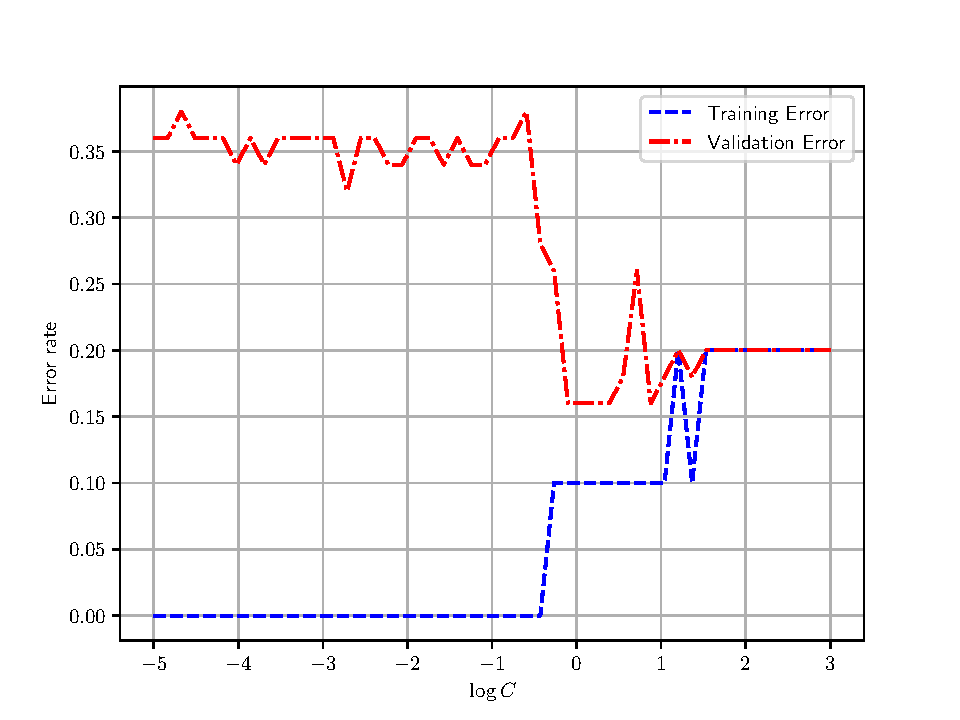
\includegraphics[width=0.9\columnwidth]{figures/overfit1.pdf}
    \end{minipage}
    \begin{minipage}{0.39\textwidth}
        \raggedleft
        \caption{
            \label{fig:weight_decay}
            Training and test errors with respect to the weight decay
            coefficient. Notice that the test error grows back even when the
            training error is $0$ as the weight decay coefficient decreases.
        }
    \end{minipage}
\end{figure}

\begin{figure}
    \centering
    \hfill
    \begin{minipage}{0.49\textwidth}
        \centering
        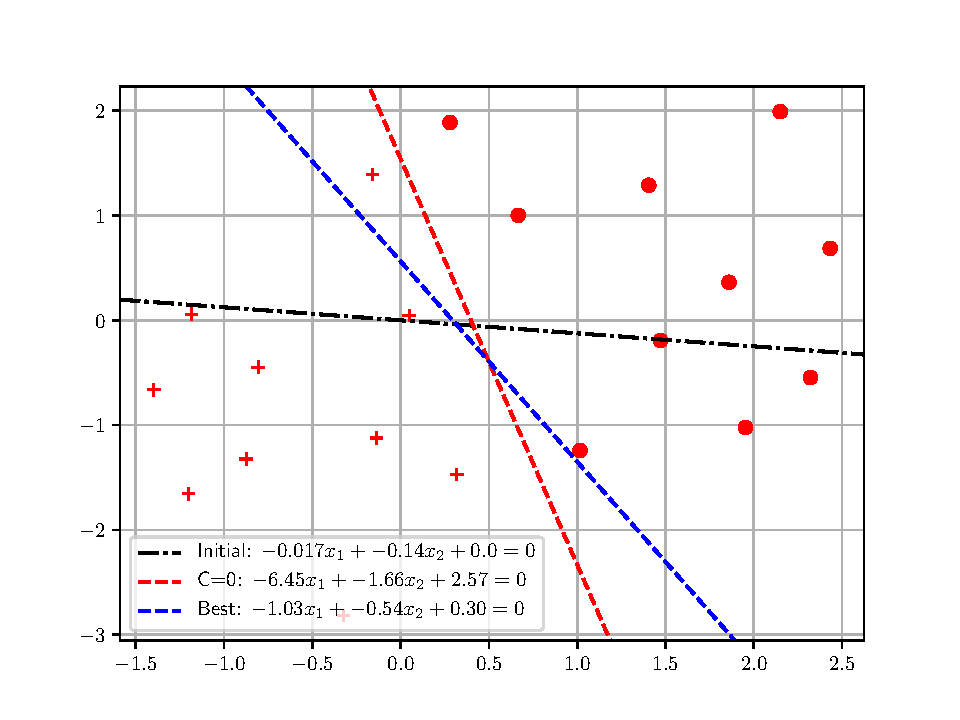
\includegraphics[width=\columnwidth]{figures/overfit2_tra.pdf}
        (a) Training Set
    \end{minipage}
    \hfill
    \begin{minipage}{0.49\textwidth}
        \centering
        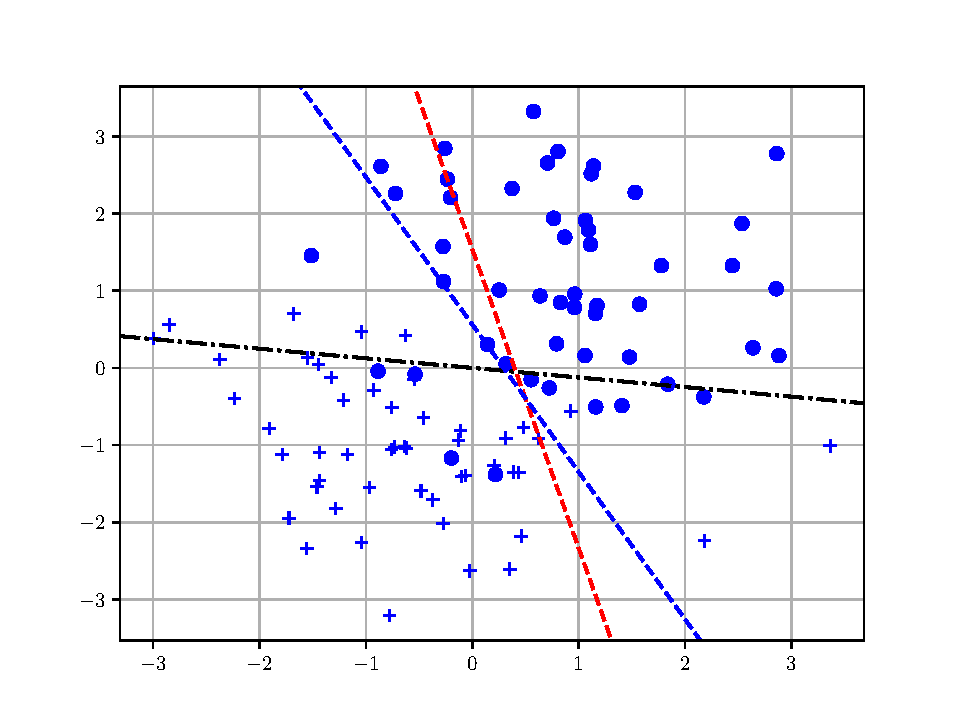
\includegraphics[width=\columnwidth]{figures/overfit2_tes.pdf}
        (b) Validation Set
    \end{minipage}

    \caption{
        \label{fig:overfit}
        Both solutions of logistic regression perfectly fit the training set
        regardless of whether weight decay regularization was used. However, it
        is clear that the model with the optimal weight decay coefficient
        ({\color{blue} blue line})
        classifies the test set better. 
    }

\end{figure}

\paragraph{Example} 

In this example there are 20 training pairs and 100 validation pairs. We search
for the best regularization coefficient, or corresponding hypothesis sets, over
the set of 50 equally-spaced $\log C$ from $-5$ to $3$. We plot how the training
and validation errors (0-1 loss) change with respect to the regularization
coefficient $C$ (or equivalently $\log C$) in Fig.~\ref{fig:weight_decay}. It is
clear from the plot that as the regularization strength weakens ($\log C \to
-\infty$) the training error drops to zero. On the other hand, the validation
error decreases until $\log C = 0$, but from there on, increases, which is a
clear evidence of overfitting. 

In Fig.~\ref{fig:overfit}, we see the difference between the support vector
machines found using $C=0$ (no regularization, red dashed line) and $\log C=0$
(best regularization according to the validation error, blue dashed line). The
red dashed decision boundary, which corresponds to the support vector machine
without any regularization, classifies all the training input vectors perfectly,
while the blue dashed decision boundary fails to classify one training input
vector near $(-0.1, 1.3)$ correctly. However, when we consider the validation
input vectors, the picture looks different. A better machine is now the
regularized support vector machine. 

\section{Multi-Class Classification}

So far, we have considered a {\it binary} classification only. In reality, there
are often more than two categories to which an input vector belongs.  It is
indeed interesting to build a machine that can tell whether an object of a
particular type, such as a dog, is in a given image, but we often want our
machine to be able to classify an object in a given image into one of many
object types. That is, we want our machine to answer ``what is in an image?''
rather than ``is a dog in an image?'' A slightly different formulation of the
same question is ``which of the following animals does this image describe, dog,
cat, rabbit, fish, giraffe or tiger?'' This kind of problem is a {\it
multi-class classification}. Instead of two possible categories as in binary
classification, now each input vector may belong to one of more than two
categories. 

Let us start from logistic regression in Sec.~\ref{sec:logreg}. We already
learned that the logistic regression classifier outputs a Bernoulli distribution
over two possible categories--negative and positive. We extend it so that the
logistic regression classifier is now returning a distribution over $K$-many
possible categories 
\begin{align}
    \label{eq:catset}
    \mathcal{C} = \left\{ 0, 1, \ldots, K \right\}.
\end{align}

First, we must decide what kind of distribution, other than Bernoulli
distribution, we should use. In this case of multi-class classification, we use
a categorical distribution. The categorical distribution is defined over a set
of $K$ events (equivalent to $K$ categories in our case) with a set of $L$
probabilities $\left\{ p_1, \ldots, p_K \right\}$. $p_k$ is the probability of
the $k$-th event happening, or the input vector belonging to the $k$-th
category. As usual with any other probability, those probabilities are
constrained to sum to $1$, i.e.,
\begin{align*}
    \sum_{k=1}^K p_k = 1.
\end{align*}

Now given an input vector $\vx$, we should let our new multi-class classifier
output this categorical distribution. This is equivalent to building a machine
that takes as input a vector $\vx$ and outputs $K$ probabilities that sum to
$1$. In order to do so, we turn the $d$-dimensional input vector
into a $K$-dimensional vector by
\begin{align*}
    \va = \mW \tilde{\vx},
\end{align*}
where $\tilde{\vx}$ is as before $\left[ \vx; 1 \right]$. $\mW$, to which we
refer as a weight {\it matrix}, is a $K \times d$-dimensional matrix. Do you see
how it has changed from a weight vector earlier to a weight matrix now?

We have $K$ real numbers in $\va$. These numbers however are not constrained,
meaning that their sum is not $1$, and that some of them may even be negative.
Let us now turn this $K$ numbers into $K$ probabilities of a categorical
distribution. First, we make them positive by exponentiating each of them
separately. That is,
\begin{align*}
    \va^+ = \exp(\va) > 0.
\end{align*}
Then, we force those $K$ positive numbers to sum to 1 by
\begin{align}
    \label{eq:multlog_out}
    \vp = \frac{1}{\sum_{k=1}^K a^+_k} \va^+.
\end{align}
That was easy, right? This transformation--exponentiation followed by
normalization-- is called {\it softmax} \cite{Bridle1990}. 

\paragraph{Hypothesis Set} 

This new machine, often called {\it multinomial logistic regression}, is fully
characterized by the weight matrix $\mW$. In other words, our hypothesis set is
a set of all $K$-by-$d$ real-valued matrices. 

\paragraph{Distance} 
We define the distance function similarly to how we did with logistic
regression. That is, it is the negative log-probability of the correct category
returned by the reference machine $M^*$:
\begin{align}
    \label{eq:multlog_dist}
    D(M^*(\vx), M, \vx) = -\log p(C=M^*(\vx) | \vx) = -\log p_{M^*(\vx)}.
\end{align}
I used $p_{M^*(\vx)}$ to denote the $M^*(\vx)$-th probability value stored in
$\vp$, which is by our definition of the machine the probability of the correct
category predicted by our machine.  Let's expand it a bit further:
\begin{align*}
    D(y^*, M, \vx) &= -\log p_{M^*(\vx)} \\
                   &= -a_{y^*} + \log \sum_{k=1}^K \exp(a_k).
\end{align*}

\paragraph{Gradient of the Distance}

As we have done so with logistic regression and support vector machines earlier,
we need to compute the gradient of the distance function in
Eq.~\eqref{eq:multlog_dist} with respect to the weight matrix.\footnote{
    The full derivation is left for you as a {\bf homework assignment}.
}

We will do this
for each row of the weight matrix separately. First, we consider the $y^*$-th
row vector, that corresponds to the correct class outputted by the reference
machine: 
\begin{align*}
    \frac{\partial D(y^*, M, \vx)}{\partial \vw_{y^*}} =&
    -\frac{\partial}{\partial \vw_{y^*}} \left(
        \vw_{y^*}^\top \tilde{\vx} - \log \sum_{k=1}^K \exp(a_k)
    \right) \\
    =& -( 1 - p(C=y^* | \vx)) \tilde{\vx}.
\end{align*}
Similarly, we can compute the gradient of the distance function with respect to
the weight vector that corresponds to any other incorrect class $y \in \left\{1,
\ldots, K \right\} \backslash \left\{ y^* \right\}$:
\begin{align*}
    \frac{\partial D(y^*, M, \vx)}{\partial \vw_{y}} =&
    -\frac{\partial}{\partial \vw_{y}} \left(
        \vw_{y}^\top \tilde{\vx} - \log \sum_{k=1}^K \exp(a_k)
    \right) \\
    =& -( 0 - p(C=y | \vx)) \tilde{\vx}.
\end{align*}

We can combine them together into a single vector equation:
\begin{align*}
\nabla_{\mW} D(y^*, M, \vx) =
    -
    \left( 
        \vy^* - \vp
    \right) \tilde{\vx}^\top,
\end{align*}
where 
\begin{align}
    \label{eq:onehot}
    \vy^* = 
    \left[ 
        \begin{array}{c}
            0, \\
            \vdots, \\
            1, \\
            \vdots, \\
            0
        \end{array}
    \right]
    \begin{array}{c}
         \\
         \\
         \leftarrow y^*\text{-th row} \\
         \\
         \\
    \end{array}
\end{align}
is an {\it one-hot vector} corresponding to a desired output, and $\vp$ is the
actual output from the multinomial logistic regression from
Eq.~\eqref{eq:multlog_out}.

This equation above reminds us of the learning rule of logistic regression (and
naturally that of perceptron.) See for instance Eq.~\eqref{eq:grad_logreg_dist}
as a comparison. Both rules (logistic regression and multinomial logistic
regression) have a multiplicative term in the front, and that multiplicative
term is a difference between the predicted output (or the predicted conditional
distribution over the categories given an input vector) and the desired output
generated by the reference machine.

For the row vector of the weight matrix corresponding to the correct category
$y^*$, this learning rule will add the input vector (augmented with an extra
one) to the this vector so that they would align better. On the other hand, for
any other category, the learning rule will subtract the input vector instead to
make them less aligned. The degree to which the input vector is subtracted is
decided based on how well the reference machine and our machine agree.  Learning
terminates, when the multinomial logistic regression puts all the probability
mass ($1$) to the correct class. 

\section{What does the weight vector tell us?}
\label{sec:weight}

Before we move on to more advanced topics, let us briefly discuss about what the
weight vector or matrix tells us. In a standard setting of binary
classification, each component $x_j$ of an input vector $\vx$ has a
corresponding weight value $w_j$. When this associated weight value is close to
$0$, what does it mean? It means that this $j$-th component does not matter!
This is easy to verify by looking at the score function we defined in
Eq.~\eqref{eq:lin_score} which can be rewritten as
\begin{align*}
    s(y, \vx; M) = y \vw^\top \tilde{\vx} = 
    y \left( \sum_{j=1}^{d} w_j x_j + w_{d+1} \right).
\end{align*}
Let's consider the $k$-th component of the input vector:
\begin{align*}
    s(y, \vx; M) = 
    y \left( 
        \sum_{j=1}^{k-1} w_j x_j + 
        w_k x_k +
        \sum_{j'=k+1}^{d} w_{j'} x_{j'} + 
    w_{d+1} \right),
\end{align*}
which is equivalent to the equation below, if $w_k=0$.
\begin{align*}
    s(y, \vx; M) =&
    y \left( 
        \sum_{j=1}^{k-1} w_j x_j + 
        \underbrace{w_k x_k}_{\mathclap{=0\text{ if }w_k=0}} +
        \sum_{j'=k+1}^{d} w_{j'} x_{j'} + 
    w_{d+1} \right)
    \\
    =& 
    y \left( 
        \sum_{j=1}^{k-1} w_j x_j + 
        \sum_{j'=k+1}^{d} w_{j'} x_{j'} + 
    w_{d+1} \right).
\end{align*}
This is as if our input vector never had the $k$-th component to start with. 

Along the same line of reasoning, we can see that the magnitude of each weight
value $\left| w_k \right|$ roughly corresponds to how sensitive the output of a
machine to the change in the value of the $k$-th component of the input vector
$x_k$. Can we make it slightly more precise by defining the sensitivity more
carefully? Indeed, we can. The sensitivity of the output of our machine,
$\vw^\top \tilde{\vx}$ with respect to a single input component $x_k$ is
precisely the definition of the partial derivative of the output with respect to
the input component. That is,
\begin{align*}
    \frac{\partial \vw^\top \tilde{\vw}}{\partial x_k}
    =& \frac{\partial}{\partial x_k} \left(
    \sum_{j=1}^{k-1} w_j x_j + 
    w_k x_k +
    \sum_{j'=k+1}^{d} w_{j'} x_{j'} \right) \\
    =& \frac{\partial w_k x_k} {\partial x_k} \\
    =& w_k.
\end{align*}
This definition of sensitivity via partial derivative will become handy in the
later part of the course.

In other words, we can understand which components of the input vector are
meaningful for or have high influence on the output of our machine by inspecting
the weight vector. For an example of inspecting the weight vector, or matrix in
the case of multi-class classification, see
\url{https://github.com/nyu-dl/Intro_to_ML_Lecture_Note/blob/master/notebook/Weight%20Analyzer.ipynb}.

\alert{TODO: Add some explanation going through the example}


\section{Nonlinear Classification}

So far in this course, we have looked at a linear classifier which defines a
hyperplane ($\vw^\top \tilde{\vx} = 0$) that partitions the input space into two
partitions. Clearly this type of classifier can only solve linearly separable
problems. A famous example in which a linear classifier fails is exclusive-OR
(XOR) problem shown in Fig.~\ref{fig:perceptron_xor}. In this section, we
discuss how to build a classifier for problems which are not linearly separable.

\begin{figure}
    \centering
    \begin{minipage}{0.6\textwidth}
        \centering
        \includegraphics[width=\columnwidth]{figures/perceptron_failure.pdf}
    \end{minipage}
    \begin{minipage}{0.39\textwidth}
        \caption{
            \label{fig:perceptron_xor}
            If the problem is not linearly separable as in the case shown, a
            linear classifier, such as perceptron, fails miserably. This is a
            famous example of a exclusive-or (XOR) problem (with noise.)
        }
    \end{minipage}
\end{figure}

\subsection{Feature Extraction}

We have so far assumed that an input vector $\vx$ is somehow given together with
data. Is this assumption reasonable? Let us think of what kind of data we run
into in practice. For instance, in the example of intrusion detection system
from earlier sections, the input to a machine is not a vector but a picture
taken by a camera installed at the front of the store. In the case of building a
machine that categorizes a document, the input to a machine is again not a
vector but a long list of words. If we are building a machine for detecting
violent scenes from a movie, our machine takes as input a video not a single,
flat vector. What all these examples suggest is that we need one more step in
addition to what we have discussed as a full pipeline of machine learning. That
is the step of feature extraction, or sometimes called feature engineering.

Let us introduce another symbol $\mathcal{X}$ to denote the original input which
could be anything from a colour image, video clip to a social network of a
person. Then, the feature extraction stage can be thought of as a function
$\phi$ that maps from this arbitrary original input $\mathcal{X}$ to a
corresponding input vector $\vx$. That is,
\begin{align*}
    \vx = \phi(\mathcal{X}).
\end{align*}

Why is this process called {\it feature extraction}? That is because the
function $\phi$ can be thought of as extracting $d$-many characteristics of the
original input $\mathcal{X}$. We extract features out of a given input
$\mathcal{X}$ and build the corresponding input vector $\vx \in \RR^d$.

\paragraph{Example: Bag-of-Words Representation}

Let us consider an example of document categorization we learned about earlier.
What is a property of a given document that largely determines the category or
topic of the document? One thing that immediately comes to our mind is the
existence of category-related words. For instance, if a word ``hockey'' is
mentioned in the document, it is highly likely that it is a document about
sports, and more specifically about hockey rather than baseball. Perhaps, it is
also important how frequently such a word appeared in the document. If the word
``baseball'' appeared ten times more than the word ``baseball'', the topic of
the document is likely ``hockey'' rather than ``baseball'', even though the word
``baseball'' appeared. 

This observation leads us to use a so-called bag-of-words (BoW) feature
representation of a document for document categorization. As the name suggests,
this representation puts all the words in a given document into a bag and counts
how often each word appeared in the document, ignoring any order among those
words. This is equivalent to turning each word into a one-hot vector from
Eq.~\eqref{eq:onehot} and sum them into a single vector. In order to do so, we
will first build a vocabulary of all unique words in all the document from a
training set (again, do not touch any test document!), which is similar to
building a category set from Eq.~\eqref{eq:catset}. We then transform a document
into a sequence of one-hot vectors $w_i$'s, and sum all those one-hot vector to
obtain a bag-of-words vector:
\begin{align*}
    \vx = \sum_{i=1}^{|\mathcal{X}|} w_i,
\end{align*}
where $|\mathcal{X}|$ denotes the length, or the number of words, of the
document $\mathcal{X}$. This BoW vector $\vx$ can be used with any machine
learning algorithm, such as any of the classifiers we have learned so far.

\begin{figure}
    \centering
    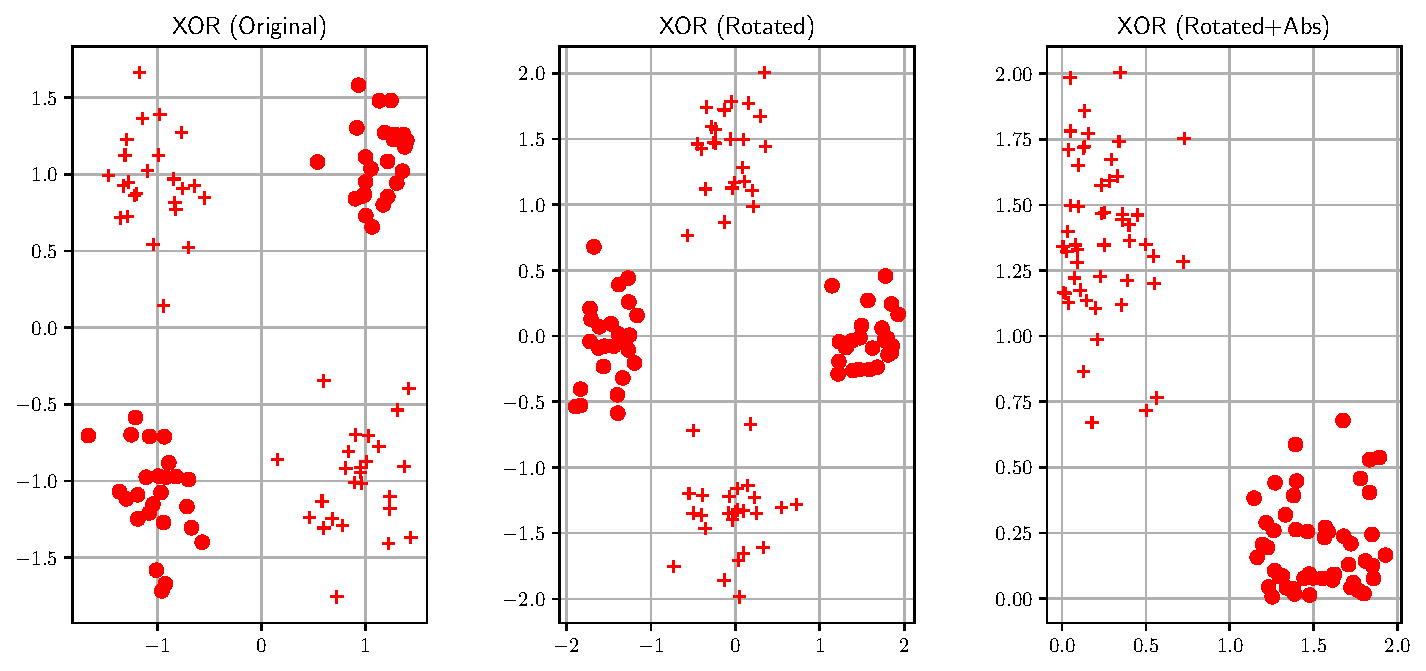
\includegraphics[width=\columnwidth]{figures/xor_transform.pdf}

    \caption{
        \label{fig:xor_transformed}
        The XOR problem in the original coordinate system (left) is not linearly
        separable, but as shown in the right panel, it become linearly
        separable by transforming the space (center and right). See the main
        text for more details.
    }
\end{figure}

\paragraph{Linear Separable Feature Extraction}

Feature extraction serves two purposes. The first purpose is to build a
fixed-dimensional vector $\vx$ from an arbitrary input $\mathcal{X}$, of which
an example was to build a bag-of-word vector from a document of arbitrary
length. The second purpose is to make a given dataset {\it easier} for a
classifier, or any other {\it linear} machines. More specifically for the case
of classifiers we have learned so far, the goal of feature extraction is to make
a dataset {\it linearly separable}, even when it is not so in the original input
$\mathcal{X}$ space. 

Let us go back to the example of XOR problem from earlier. In its original form,
the XOR problem is not solvable by a linear classifier, because the positive and
negative classes are not linear separable, meaning that there is no 1-D
hyperplane (line) that separates the examples into the positive and negative
classes. The question is then: can we somehow transform the original input--a
vector in a 2-D space-- so that the transformed data is linear separable?

First, let us rotate the whole space, or every single point in the space,
clock-wise by 45 degrees. This can be done by first defining a rotation matrix
as
\begin{align*}
    R(\theta) = \left[
        \begin{array}{c c}
            \cos \theta & -\sin \theta \\
            \sin \theta & \cos \theta
        \end{array}
    \right],
\end{align*}
where $\theta$ is in radian ($\text{rad}(45^\circ) \approx 0.785$). We then
rotate each point in the space by
\begin{align*}
    \vx^r = R(\text{rad}(45^\circ)) \vx.
\end{align*}
The XOR problem after this rotation is illustrated in the center panel of
Fig.~\ref{fig:xor_transformed}. 

The problem is however not linearly separable yet. Let us then further apply one
more transformation. That is, we will take the absolute value of each element of
the resulting, rotate vector:
\begin{align*}
    \vx^{ra} = \left[ 
        \begin{array}{c}
            |x^r_1| \\
            |x^r_2|
        \end{array}
    \right].
\end{align*}
Effectively, we fold the four quadrants of the rotated space into the first
quadrant (the top-right one), and the resulting space is now linearly separable
as shown in the right panel of Fig.~\ref{fig:xor_transformed}.  Within this new
transformed space, the XOR problem, which was not linearly separable, is now
linearly separable, and we can use any of the linear classification machines we
have learned earlier. 

This is a great news! Apparently, we can find a set of features--the elements in
an input vector $\vx$-- that turn a problem, which is not linearly separable in
its original form, into a linearly separable one. As long as we can find such a
transformation, or a sequence of them, we are pretty much solve any
classification problem.  

Unfortunately, it is  often impossible to find such a transformation manually,
because the original inputs or the original feature vectors are almost always
high-dimensional. In the remainder of this section, we will discuss how we can
automate such a procedure. 

\subsection{$k$-Nearest Neighbours: Fixed Basis Networks}

Let us consider another transformation for the XOR problem above. We start with
selecting four points in the space that correspond to 
\begin{align*}
    &\vr^1 = [-1, -1] \\
    &\vr^2 = [1, 1] \\
    &\vr^3 = [-1, 1] \\
    &\vr^4 = [1, -1] \\
\end{align*}
to which we refer as {\it basis vectors}. With these basis vectors, we will
transform each two-dimensional input vector $\vx$ into a four-dimensional vector
$\phi(\vx)$ such that
\begin{align}
    \label{eq:rbf}
    \phi_i(\vx) = \exp\left( -(\vx - \vr^i)^2 \right).
\end{align}
This is equivalent to saying that the $i$-th element of the transformed vector
$\phi(\vx)$ is inversely proportional to the distance between the input vector
$\vx$ and the $i$-th basis vector. 

This function is often called a (Gaussian) {\it radial basis function}. This
function's output is bounded between $0$ and $1$. The output is closer to $1$,
when the input vector $\vx$ is close to the basis vector $\vr$, but converges to
$0$ as the distance between them grows. 

In this newly transformed space, the XOR problem is linearly separable. How do
we confirm this? We can either train a linear classifier, such as the ones we
have learned so far in the course, or manually find a weight vector $\vw \in
\RR^5$ that solves the problem perfectly. Let us try the latter, based on the
intuition we built from Sec.~\ref{sec:weight}.

We first observe that any input vector that is close to one of the first two
basis vectors $\vr^1$ and $\vr^2$ should be classified as a positive class, and
an input vector closer to either $\vr^3$ or $\vr^4$ should be classified as a
negative class. In other words, any positive input vector would have either the
first or second element of the transformed vector close to 1, while any negative
input vector close to 0. For the third and fourth elements, they would have a
value close to 1, if the original input vector is negative, and close to 0
otherwise. 

Based on this observation, we can easily notice that the following weight vector
will perfectly solve the problem:\footnote{
    It is a {\bf homework assignment} for you to show that this weight vector
    solves the XOR problem in the new space. 
}
\begin{align*}
    \vw = \left[ 1, 1, -1, -1, 0 \right]^\top.
\end{align*}

The weight vector above can be written alternatively as 
\begin{align}
    \label{eq:w_rbf}
    \vw = \left[ y^1, y^2, y^3, y^4, 0\right]^\top,
\end{align}
where $y^i$ is the class label (-1 or 1) of the $i$-th basis vector.\footnote{
    It is your {\bf homework assignment} to find such a weight vector when the
    class labels are given as $0$ and $1$.
}
In other words, the input vector $\vx$ belongs to the class to which the {\it
nearest} basis vector belongs. 

Let us generalize this idea by assuming that we have $K$ basis vectors and their
corresponding labels:
\begin{align*}
    \left\{ (\vr^1, y^1), \ldots, (\vr^K, y^K) \right\}.
\end{align*}
Each input vector $\vx$ is transformed into
\begin{align}
    \label{eq:W_rbf}
    \phi(\vx) = \left[ 
        \begin{array}{c}
            \exp\left( -(\vx - \vr^1)^2 \right)  \\
            \vdots \\
            \exp\left( -(\vx - \vr^K)^2 \right)  \\
        \end{array}
    \right]
\end{align}

In the case of binary classification, the optimal weight vector is given in
Eq.~\eqref{eq:w_rbf}. In multi-class classification, the weight matrix $\mW$ can
be constructed as
\begin{align*}
    \mW = \left[
        \vy^1, \ldots, \vy^K
    \right],
\end{align*}
where $\vy^i$ is the one-hot vector corresponding to the class to which the
$i$-th basis vector belongs (see Eq.~\eqref{eq:onehot}.) Again, it is left for
you as a {\bf homework assignment} to show that this construction of the weight
matrix solves the problem of multi-class classification.

Suddenly the problem of finding a linearly separable transformation has become a
problem of finding a set of good basis vectors and their own classes. Of course,
now a big question is what these good basis vectors. An even bigger question is
how we know to which class each of those basis vectors belongs. After all, the
whole point of classification is to figure out this latter question.

\paragraph{$k$-Nearest Neighbours}

We can push this idea to the extreme by declaring each and every input vector in
a training set as basis vectors. Furthermore, instead of building a linear
classifier in the transformed space (using all the training input vectors as
basis vectors,) we can simply use the class label of the nearest basis vector,
or more conventionally {\it nearest neighbour}. 

This can be written down more formally by first defining as many basis vectors
as there are training examples. That is,
\begin{align*}
    \vr^i = \vx_i,
\end{align*}
where $\vx^i$ is the $i$-th input vector in a training set. Then, each input
vector is transformed in two stages. First, we use the radial basis function to
get $\phi(\vx)$ as done in Eq.~\eqref{eq:rbf}. Second, we turn the resulting
vector into an one-hot vector by setting the element with the largest value to
$1$ and all the others to $0$:
\begin{align*}
    \phi'(\vx) = \argmax(\phi(\vx)).
\end{align*}
The weight matrix is constructed as before in Eq.~\eqref{eq:W_rbf}.  In
practice, none of these formal steps is necessary. All that is needed is to find
the nearest neighbour from a training set given an arbitrary (test) vector, and
return the class of the nearest neighbour. We call this classifier a {\it
nearest-neighbour classifier}.

The nearest-neighbour classifier can be written down in a single equation:
\begin{align*}
    \argmin_{(\vx, y) \in D_{\text{tra}}} \| \vx - \vx' \|^2,
\end{align*}
where $\vx'$ is a new input vector of which label must be found. Note that it is
not necessary to use the Euclidean distance $\| a - b \|^2$, and any distance
function may be used instead.

\begin{figure}[t]
    \begin{minipage}{0.32\textwidth}
        \centering
        \includegraphics[width=\columnwidth]{figures/knn_k1.pdf}

        (a) $k=1$
    \end{minipage}
    \hfill
    \begin{minipage}{0.32\textwidth}
        \centering
        \includegraphics[width=\columnwidth]{figures/knn_k5.pdf}

        (b) $k=5$
    \end{minipage}
    \hfill
    \begin{minipage}{0.32\textwidth}
        \centering
        \includegraphics[width=\columnwidth]{figures/knn_k20.pdf}

        (c) $k=20$
    \end{minipage}

    \caption{
        \label{fig:knn}
        The effect of varying $k$ in $k$-nearest-neighbour classifier. We
        observe that the decision boundary becomes {\it smoother} as $k$
        increases, which suggests that a large $k$ corresponds to having a
        stronger regularization term.
    }
\end{figure}

The nearest-neighbour classifier is rarely used in practice. Instead, it is more
common to use its variant, called a {\it $k$-nearest-neighbour} (KNN)
classifier.  Unlike the nearest-neighbour classifier, the KNN classifier selects
$k$ nearest input vectors from a training set given a new input vector, and lets
them vote on which category this new vector belongs to. The nearest-neighbour
classifier is thus a special case of the KNN classifier, where $k$ is fixed to
$1$. 

Increasing $k$ has the effect of regularization, similarly to the weight decay
regularization term, or the max-margin regularization term from support vector
machines (see Eq.~\eqref{eq:svm}~(a).) When $k=1$, the empirical cost on a
training set is perfect by definition, but this nearest-neighbour classifier is
susceptible to outliers or noise. Imagine a case where one negative input vector
was accidentally placed in the middle of a cluster\footnote{
    A cluster refers to a group of closely located input vectors. 
}
of positive input vectors. The nearest-neighbour classifier would assign any
input vector in a small region around this negative input vector to a negative
class, although it is quite clear that this training example is an outlier, or
was labelled incorrectly. This behaviour, which is a classical example of
overfitting, is easily mitigated by using $k > 2$, as this would ignore such an
outlier training example. On the other hand, we can also think of a case where
$k = |D_{\tra}|$, in which case any new input vector would be assigned to a
majority class, and such a KNN classifier wouldn't be able to correctly classify
any training input vector belonging to a minority class. The latter case is
considered {\it over-regularized} or {\it under-fitted}. 


\subsection{Radial Basis Function Networks}

The most obvious weakness of the KNN classifier is that it requires (a) a large
storage (since it must maintain the entire training set,) and (b) a sweep
through the entire training set (unless some smart indexing with an appropriate
approximation strategy is used.) This becomes more severe, as the size of a
training set grows (which is precisely what is happening everyday,) and if there
is a computational constraint in run-time (such as when run on a mobile phone.) 

A radial basis function (RBF) network overcomes this weakness of the KNN
classifier by selecting only a small number of basis vectors, according to
memory and computational constraints. Of course, as we discussed earlier, how
should we choose such basis vectors?

\todo{}

\subsection{Deep Learning: Adaptive Basis Networks}

\begin{figure}
    \centering
    \begin{minipage}{0.6\textwidth}
        \centering
        \includegraphics[width=\columnwidth]{figures/adaptive_basis1.png}
    \end{minipage}
    \begin{minipage}{0.39\textwidth}
        \caption{
            \label{fig:feature_extraction}
            The goal of adaptive basis networks is to find a parametrized
            mapping from the original input space $\vx \in \mathbb{R}^d$ to
            another space $g(\vx) \in \mathbb{R}^q$ that makes the problem
            linearly separable. 
        }
    \end{minipage}
\end{figure}

\paragraph{Adaptive Basis Networks and Representation Learning}

\todo{}


\section{Kernel Support Vector Machines$^\star$}

\section{Decision Tree$^\star$}

\section{Ensemble Methods$^\star$}


\chapter{Regression}
\label{sec:regression}

We have so far considered a problem of classification, where the output of a
machine $M$ is constrained to be a finite set of discrete labels/classes. In
this section, we consider a {\it regression} problem in which case the machine
outputs an element from an infinite set.\footnote{
    This definition however is not universal, in that even when the output is
    from a finite set, the problem is sometimes called regression if there
    exists natural ordering of labels.
} A general setup of the problem remains largely identical to that from
Sec.~\ref{sec:supervised_learning}, meaning that it is probably a good idea to
re-read that section at this point.  In the context of regression, we will
particularly focus on framing the whole problem as probabilistic modelling. 

\section{Linear Regression}

\subsection{Linear Regression}

As we have done with classification, we will start with considering {\it linear}
regression. In linear regression, our machine $M$ is defined as 
\begin{align*}
    M(\vx) = \vw^\top \tilde{\vx},
\end{align*}
where we use $\tilde{\vx}$ to denote the input vector with an extra $1$ attached
at the end. 


\subsection{Regularization and Prior Distributions}


\section{Bayesian Linear Regression and Gaussian Process Regression}

\subsection{Bayesian Approach to Machine Learning}

\begin{figure}[t]
    \centering
    \begin{minipage}{0.48\textwidth}
        \centering
        \includegraphics[width=\columnwidth,clip=True,trim=50 0 50
        0]{figures/bayes_logreg.pdf}

        (a)
    \end{minipage}
    \hfill
    \begin{minipage}{0.48\textwidth}
        \centering
        \includegraphics[width=\columnwidth,clip=True,trim=50 0 50
        0]{figures/bayes_linreg_mlp.pdf}

        (b)
    \end{minipage}

    \caption{
        \label{fig:bayes_logreg}
        (a) Bayesian logistic regression, and (b) Bayesian multilayer
        perceptron. Both of them were done with ``ensemble samplers with affine
        invariance'' \cite{goodman2010ensemble} using Python emcee available at
        \url{http://dan.iel.fm/emcee/current/}. 
    }
\end{figure}


\subsection{Gaussian Process Regression$^\star$}


\chapter{Dimensionality Reduction}
\label{chap:dimred}

\section{Unsupervised Learning: Problem Setup}

Unsupervised learning is a weird, but fascinating problem. Unlike supervised
learning in which a machine was defined as a transformation of an input vector
$\vx$, a machine $M$ in unsupervised learning {\it scores} an input vector
according to how likely that vector is. If an input vector $\vx$ is likely, the
output of the machine $M(\vx)$ would be higher, and otherwise lower. The use of
the term {\it score} should remind you of our earlier discussion on
classification, and it is only natural because there is a strong connection
between supervised learning and unsupervised learning. This connection is
apparent when we consider $\vx$ as a concatenation of an input vector $\vx$ and
its corresponding label $y$. Then, with a machine $M$ trained by unsupervised
learning, we can classify any given input vector by
\begin{align*}
    \hat{y} = \argmax_y M(\left[ \vx; y\right]).
\end{align*}
We can similarly perform regression in this framework.  

This capability of scoring an input vector allows us to use it for {\it outlier
detection} as well. Given an input vector $\vx$, we will declare it as an
outlier if its score is lower than a certain, predefined threshold:
\begin{align*}
    \vx\text{ is an outlier if }M(\vx) < \tau.
\end{align*}
The threshold $\tau$ may be found by any of the validation techniques we
discussed in Sec.~\ref{sec:validation}.  Furthermore, we can even {\it generate}
a novel input vector by finding an input vector that maximizes the score given
by the model:
\begin{align*}
    \hat{\vx} = \argmax_{\vx} M(\vx).
\end{align*}

\todo{}




\subsection{Naive Bayes Classifier}

\todo{}

\section{Dimensionality Reduction: Problem Setup}
\label{sec:dimred}

\section{Principal Component Anslysis}

\subsection{Minimum Reconstruction Criterion}

\subsection{Maximum Variance Criterion}

%\subsection{PCA with Missing Values$^\star$: Collaborative Filtering}

\subsection{Probabilistic Principal Component Analysis}

\paragraph{Expectation-Maximization Algorithm}

\section{Other Dimensionality Reduction Techniques$^\star$}


\chapter{Clustering}
\label{sec:cluster}

\section{Problem Setup}

\subsection{Clustering vs. Dimensionality Reduction}

\section{$k$-Means Clustering}

\section{Mixture of Gaussians$^\star$}

\section{Other Clustering Methods$^\star$}


\chapter{Sequential Decision Making}

\section{Sequential Decision Making as a Series of Classification Problems}
\todo{}


\section{Time-Series Modelling$^\star$}
\label{sec:timeseries}









\bibliographystyle{abbrv}
\bibliography{lecture_note}


\end{document}






